
%%%
%%% iTrameRA : Trame pour le Rapport d'Activité Inria 2018
%%% ------------------------------------------------------
%%%  
%%% Url de la trame : http://irabot.inria.fr/itramera?projet=visages
%%%
%%% ----------------

%%%  Nouveautés ou rappels 2018 !
%%% ----------------
%%% - Personnes : mettez à jour https://gef.inria.fr/ (assistante) pour obtenir des imports corrects pour les mots-clés et le RA
%%% - Mots-clés : mots-clés équipe et personnes à renseigner dans https://bastri.inria.fr/FichesProjets/  - Etape nécessaire pour pouvoir déposer le RA
%%% - Logiciels : à renseigner dans BIL https://bil.inria.fr/fr/catalog/listby/raweb avant l'import dans le RA. Les modifications sont à faire dans BIL, ce n'est pas possible dans le RA.
%%% - Médiation : un rubricage fin des activités vous est proposé dans la section Dissemination

%%% ------------------
%%% Ce document est un squelette de rapport d'activité  
%%% mis à jour à partir des bases de données de l'Inria
%%% (HAL pour les publis, BASTRI pour les équipes, FicheProjet pour les mots-clés, BIL pour les logiciels, l'entrepôt pour les données DPEI ...).
%%% Le rédacteur doit compléter ce document.  
%%%
%%% Marche à suivre :
%%%
%%% Récuperer l'archive tgz de 2018 et la décompresser  dans un répertoire.  
%%% Il y a un fichier tex et 3 fichiers de bibliographie (.bib) :  
%%% - visages2018.tex : le texte en latex du rapport  
%%% - visages2018.bib : les publis de l'année 2018 issues de Hal
%%% - visages_refer2018.bib : les publications de référence (c'est-a-dire les 10 publis les plus importantes
%%%   de l'équipe quelle que soit l'année)
%%% - visages_foot2018.bib : les publis placées dans les notes de bas de page (footnote) issues de votre rapport 2017
%%%
%%% Instructions pour l'écriture du RA :
%%%
%%% https://intranet.inria.fr/Vie-scientifique/Information-edition-scientifiques/Comment-rediger-le-RAweb/Rediger-le-RA-Objectifs-et-actualites
%%%
%%% Pour compiler puis déposer le rapport utiliser le serveur iRAbot :  
%%%
%%% http://irabot.inria.fr/irabot
%%%
%%% ou bien le script irabot.sh qui utilise iRAbot.
%%%
%%% Le rapport est en ANGLAIS !
%%%


\documentclass{ra2018}

%SKEL - v0.4 - 2018 (Utiliser pour les stats d'utilisation de Skel, merci de ne effacer cette ligne)

% ne pas enlever  
\renewenvironment{motscle}{\begin{xmlelement}{keywords}}{\end{xmlelement}}

%%% Par defaut sont inclus les packages : html, french, graphics et footbib  
%%% (ifthen curves soul epsf html)
%%% Le plus souvent la commande \usepackage n'est pas prise en compte  
%%% Mais si le package est calc ou fp certaines commandes sont rendues disponibles
%%% (fancyvrb)  

%%% Mettez ici les \newcommand et \def que vous voulez



%%%%%%%%%%%%%%%%%%%%%%%%%%%%%%%%%%%%%%%%%%%%%%%%%%%%%%%%%%%%%%%%%%%%%%%%%%%%%%
%%%
%%%  Information sur les données importées : Bastri
%%%
%%% L'acronyme de votre équipe et le CRI sont présentés comme dans les fiches projets.
%%% Si vous souhaitez les modifier, faites-le dans la base de gestion des fiches projets :
%%% https://bastri.inria.fr/FichesProjets/ et régénérez votre trame.

%%% Les organismes ou écoles partenaires de votre équipe, les labos auxquels
%%% vous êtes associés ainsi que thème et domaine de rattachement sont récupérés automatiquement à chaque compilation.
%%%. Ces infos sont issues de Bastri :  https://bastri.inria.fr, la base des structures de recherche Inria.
%%%
%%% Le "moreinfo" de l'équipe servira donc uniquement à préciser la localisation  
%%% quand elle est distincte du CRI (pour ceux qui le souhaitent).  
%%%
%%%%%%%%%%%%%%%%%%%%%%%%%%%%%%%%%%%%%%%%%%%%%%%%%%%%%%%%%%%%%%%%%%%%%%%%%%%%%%%%%
%%%
%%%  Information sur les données importées : Cartographie
%%% Cartographie de l'activité : chaque équipe et chaque membre d'équipe doit renseigner les mots-clés 2018 décrivant son activité dans https://bastri.inria.fr/FichesProjets/.  
%%% Le RA importe les mots-clés équipe. Ils sont visibles dans le RA *10 à 15 mn* après la validation dans https://bastri.inria.fr/FichesProjets/.  
%%% Le dépôt du RA est impossible tant que les mots-clés ne sont pas validés.
%%% Documentation intranet : https://intranet.inria.fr/Vie-scientifique/Information-edition-scientifiques/RAweb/Consignes-generales#eztoc26917_4
  
%%% Vérifiez et signalez erreurs et problèmes sur le Helpdesk : https://helpdesk.inria.fr/categories/181/submit
%%%
%%%%%%%%%%%%%%%%%%%%%%%%%%%%%%%%%%%%%%%%%%%%%%%%%%%%%%%%%%%%%%%%%%%%%%%%%%%%%%


%%% \projet{<PROJET>}{<ALT-ABRÉGÉ>}{<NOM-PROJET-EXPLICITÉ>}
%%% exemple :  
%%% \projet{EXEMPLE}{ExemplE}{Algebraic Systems for Research and Industry}  
%%%


%%%%%%%%%%%%%%%%%%%%%%%%%%%%%%%%%%%%%%%%%%%%%%%%%%%%%%%%%%%%%%%%%%%%%%%%%%
% Informations concernant l'equipe extraites de BASTRI
% Source : http://bastri.inria.fr/
% Date : jeudi 22 novembre 2018, 15:00:58 (UTC+0100)
%

\projet{VISAGES}{visages}{Vision, Action and information manaGement System in health}

%% Pour information le domaine et le theme du projet 
%% Domaine : Digital Health, Biology and Earth
%% Theme : Computational Neuroscience and Medicine


%%% CRI Inria  
%%% Sophia, ou Paris, ou Nancy, si le projet est bilocalisé : \UR{cr1,cr2} etc

\UR{Rennes}



%%%%%%%%%%%%%%%%%%%%%%%%%%%%%%

\begin{document}
\maketitle


%%% Pour ceux qui le souhaitent le moreinfo permet d'insérer un texte
%%% de 3 - 4 lignes qui indique les particularités de l'équipe.
%%% Ne doublonnez pas thème, domaine, CRI et partenariats qui sont ajoutés automatiquement.  

%%\begin{moreinfo}
%%ICI Vous pouvez ecrire du texte


%%\end{moreinfo}


%%%%%%%%%%%%%%%%%%%%%%%%%%%%%%%%%%%%%%%%%%%%%%%%%%%%
%%%
%%% Liste des modules possibles pour les sections :
%%% composition presentation fondements domaine highlights logiciels resultats contrats partenariat diffusion
%%%
%%% ex : \begin{module}{composition}
%%%
%%% \begin{module} {<SECTION>} {<NOMMODULE>} {<TITRE>}
%%%     <PERSONNES>  
%%%    [<GLOSSAIRE>]  
%%%    [<MOREINFO>]  
%%%    [<RESUME>]  
%%%    <CORPS>
%%% \end{module}
%%%
%%%
%%% NOMMODULE est un identifiant unique pour repérer le module,
%%% aussi chaque module doit en avoir un NOMMODULE différent.  
%%%
%%% \begin{module}{logiciels}{calcul-formel}{Sofrware aspects of Computer Algebra}
%%%  \begin{participants}
%%%  format: \pers <PRENOM> [<PARTICULE>] <NOM> [<MOREINFO>]
%%%        \pers{Jean}[de]{La Fontaine}[1621-1695],
%%%        \pers{Cecil Blount}{De Mille}
%%%  \end{participants}
%%%  \begin{glossaire}
%%%       \glo{backward combatability}{A property of hardware or software
%%%   ... but activeliy... }
%%%  \end{glossaire}
%%%  \begin{abstract}
%%%       Le joli résumé que voilà
%%%  \end{abstact}  
%%%  This is a very short module with a hypertext link to the
%%%  \href{http://www.eps.mcgill.ca/jargon/jargon.html}{Jargon File}.
%%% \end{module}
%%%
%%%%%%%%%%%%%%%%%%%%%%%%%%%%%%%%%%%%%%%%%%%%%%%%%%%%%%%%%%%%%%%%%%%%%


%%%%%%%%%%%%%%%%%%%%%%%%%%%%%%%%%%%%%%%%%%%%%%%%%%%%%%%%%%%%%%%%%%%%%
%%%
%%% Composition de l'équipe
%%%
%%% Professions possibles :
%%% Chercheur Enseignant PostDoc PhD Technique Stagiaire Assistant Visiteur CollaborateurExterieur
%%%  
%%% Utiliser le mot-clé [Habilite] pour les titulaires d'une Thèse d'État ou d'une HDR
%%%
%%%       \pers{Prénom}{Nom}{profession}[champ_libre: Employeur, Fonction, until/since, financement, info supplémentaire][Habilite]?
%%%        ...
%%%
%%% La mention "Team leader" est précisée dans le champ libre (moreinfo) et pré-remplie par l'export GEF.
%%%
%%% Dans le champ libre, si vous indiquez le grade (donnée importée si elle est dans Gef), écrivez :
%%%    
%%%   Pour DR : Senior Researcher  
%%%   Pour CR : Researcher
%%%   Pour Advanced Research position : Advanced Research position
%%%   Pour Starting Research position : Starting Research position
%%%   Pour Professeur : Professor ou Prof
%%%   Pour Maitre de conférence : Associate Professor
%%%   Pour les chercheurs émérites : Emeritus

%%%
%%%%%%%%%%%%%%%%%%%%%%%%%%%%%%%%%%%%%%%%

%%%%%%%%%%%%%%%%%%%%%%%%%%%%%%%%%%%%%%%%%%%%%%%%%%%%%%%%%%%%%%%%%%%%%%
%%%
%%% Information sur les données importées : les membres de l'équipe sont importés de GEF
%%%  
%%% Tous les membres de l'équipe doivent être dans GEF  
%%% Ajoutez et corrigez les noms dans https://gef.inria.fr et régénérez la trame.
%%% Les infos de financement viennent de la base Safin et la graphie des noms des responsables d'équipe de Bastri.
%%% La mention "Team leader" est exportée dans le champ libre (moreinfo), de même que l'employeur (à vérifier)
%%% Vérifiez et signalez erreurs et problèmes dans le Helpdesk : https://helpdesk.inria.fr/categories/181/submit
 %%%Documentation intranet : https://intranet.inria.fr/Vie-scientifique/Information-edition-scientifiques/Comment-rediger-le-RAweb/Les-sections#eztoc27554_2
%%%
%%%%%%%%%%%%%%%%%%%%%%%%%%%%%%%%%%%%%%%%%%%%%%%%%%%%%%%%%%%%%%%%%%%%%%  


%%%%%%%%%%%%%%%%%%%%%%%%%%%%%%%%%%%%%%%%%%%%%%%%%%%%%%%%%%%%%%%%%%%%%%%%%%%%%%
% Donnees  construites d'après les informations de la base GEF pour 2018
% Source : https://gef.inria.fr/
% Date : jeudi 22 novembre 2018, 15:00:58 (UTC+0100)
%

\begin{composition}
\pers{Christian}{Barillot}{Chercheur}[CNRS, Senior Researcher][Habilite]
\pers{Emmanuel}{Caruyer}{Chercheur}[CNRS, Researcher]
\pers{Julie}{Coloigner}{Chercheur}[CNRS, Researcher, from Oct 2018]
\pers{Olivier}{Commowick}{Chercheur}[Inria, Researcher]
\pers{Camille}{Maumet}{Chercheur}[Inria, Researcher]
\pers{Isabelle}{Bonan}{Enseignant}[Univ de Rennes I, Professor][Habilite]
\pers{Gilles}{Edan}{Enseignant}[Univ de Rennes I, Professor]
\pers{Jean-Christophe}{Ferré}{Enseignant}[Univ de Rennes I, Professor][Habilite]
\pers{Jean-Yves}{Gauvrit}{Enseignant}[Univ de Rennes I, Professor][Habilite]
\pers{Pierre}{Maurel}{Enseignant}[Univ de Rennes I, Associate Professor]
\pers{Sudhanya}{Chatterjee}{PhD}[Univ de Rennes I]
\pers{Mathis}{Fleury}{PhD}[Inria]
\pers{Pierre-Yves}{Jonin}{PhD}[Centre hospitalier régional et universitaire de Rennes]
\pers{Anne}{Kerbrat}{PhD}[Centre hospitalier régional et universitaire de Rennes, until Oct 2018]
\pers{Antoine}{Legouhy}{PhD}[CNRS]
\pers{Stephanie}{Leplaideur}{PhD}[Centre hospitalier régional et universitaire de Rennes]
\pers{Cédric}{Meurée}{PhD}[\_\_\_EMPLOYEUR???\_\_\_]
\pers{Maia}{Proisy}{PhD}[Centre hospitalier régional et universitaire de Rennes, until Oct 2018]
\pers{Xavier}{Rolland}{PhD}[CNRS, from Oct 2018]
\pers{Haykel}{Snoussi}{PhD}[Inria]
\pers{Raphael}{Truffet}{PhD}[Univ de Rennes I, from Oct 2018]
\pers{Corentin}{Vallée}{PhD}[Univ de Rennes I]
\pers{Élise}{Bannier}{Technique}[Centre hospitalier régional et universitaire de Rennes]
\pers{Yao}{Chi}{Technique}[Inria, until Nov 2018]
\pers{Julie}{Coloigner}{Technique}[Inria, until Sep 2018]
\pers{Benoit}{Combès}{Technique}[Inria]
\pers{Isabelle}{Corouge}{Technique}[Univ de Rennes I]
\pers{Claire}{Cury}{Technique}[Inria]
\pers{Quentin}{Duché}{Technique}[Inria]
\pers{Inès}{Fakhfakh}{Technique}[Inria, until Feb 2018]
\pers{Francesca}{Galassi}{Technique}[Inria]
\pers{Michael}{Kain}{Technique}[Inria, until Nov 2018, granted by CEA]
\pers{Florent}{Leray}{Technique}[Inria, until Feb 2018]
\pers{Giulia}{Lioi}{Technique}[Inria]
\pers{Aneta}{Morawin}{Technique}[Inria, until Aug 2018]
\pers{Mathieu}{Simon}{Technique}[Inria, until Jan 2018]
\pers{Arnaud}{Touboulic}{Technique}[Inria, until Oct 2018]
\pers{Abir}{Affane}{Stagiaire}[Univ de Rennes I, from Apr 2018 until Sep 2018]
\pers{Simon}{Butet}{Stagiaire}[Centre hospitalier régional et universitaire de Rennes, from Feb 2018 until Jul 2018]
\pers{Raphael}{Chouteau}{Stagiaire}[Univ de Rennes I, from Feb 2018 until Oct 2018]
\pers{Leonie}{Chretien}{Stagiaire}[Univ de Rennes I, from May 2018 until Aug 2018]
\pers{Rui}{Dai}{Stagiaire}[Univ de Rennes I, from Mar 2018 until Aug 2018]
\pers{Charlotte}{Laurent}{Stagiaire}[Centre hospitalier régional et universitaire de Rennes, from Feb 2018 until Aug 2018]
\pers{Solene}{Tarride}{Stagiaire}[Univ de Rennes I, from Apr 2018 until Oct 2018]
\pers{Raphael}{Truffet}{Stagiaire}[Ecole normale supérieure de Rennes, from Feb 2018 until Jun 2018]
\pers{Armelle}{Mozziconacci}{Assistant}[CNRS]
\pers{Alice}{Bates}{Visiteur}[Inria, Oct 2018]
\pers{Jean-Marie}{Batail}{CollaborateurExterieur}[Centre hospitalier régional et universitaire de Rennes, until Feb 2018]
\pers{Florence}{Le Jeune}{CollaborateurExterieur}[Univ de Rennes I]
\pers{Gabriel}{Robert}{CollaborateurExterieur}[Univ de Rennes I]
\end{composition}




%%%%%%%%%%%%%%%%%%%%%%%%%%%%%%%%%%%%%%%%%%%%%%%%%%%%%%%%%%%%%%%%%%%%%%%%%%
%%%
%%% Section presentation (Overall Objectives)
%%% On peut mettre un ou plusieurs modules.
%%%  
%%% La partie présentation du projet est issue de la section "Overall Objectives" du RAweb 2017  
%%% source : http://raweb.inria.fr/rapportsactivite/2017/visages/uid0.html
%%%
%%%Documentation intranet : https://intranet.inria.fr/Vie-scientifique/Information-edition-scientifiques/Comment-rediger-le-RAweb/Les-sections#eztoc27554_5
%%%%%%%%%%%%%%%%%%%%%%%%%%%%%%%%%%%%%%%%%%%%%%%%%%%%%%%%%%%%%%%%%%%%%%%%%%


%%%%%%%%%%%%%%%%%%%%%%%%%%%%%%%%%%%%%%%%%%%%%%%%%%%%%%%%%%%%%%%%%%%%%%%%%%%%%%
% Présentation du projet issues des informations du RAweb 2017
% Source : http://raweb.inria.fr/rapportsactivite/RA2017/visages/uid3.html
% Date : jeudi 22 novembre 2018, 15:00:58 (UTC+0100)
%


        \begin{module}{presentation}{presentation}{Overall objectives}
        \label{sec:overall}
        %%%%%%%\begin{motscle}
        \emph{
          Medical Imaging, 
          Neuroinformatics, 
          Neuroimaging, 
          Medical Image Computing, 
          Modeling of normal and pathological behavior of the human brain,
          e-health \& HealthGrids
        }
        %%%%
        %
        %
%\end{motscle}
        
        The Unit/Project \textsc{VisAGeS} U1228 is a research team jointly affiliated to
        INSERM (National Institute of Health and Scientific Research), Inria (National
        Institute of Research in Computer Sciences and Automation) and IRISA / UMR CNRS
        6074, University of Rennes I. We are located in Rennes, France on both medical
        and sciences campus. The team was created in 2005. Our ambition is to set
        up a multidisciplinary team merging researchers in image processing and medical
        doctors.  The goal of \textsc{VisAGeS} is to constitute a multidisciplinary
        team. Even though, research in medical imaging could find motivation and
        recognition based on methodological breakthroughs alone, the ultimate goal,
        when dealing with medical imaging research, is to make the clinical practice
        benefit from the basic and applied research, while keeping the excellence of
        the methodological research. This objective entails the creation of teams
        encompassing clinical and scientific researchers to design and conduct research
        projects together. Our aim through the past period was to build a research team
        able to perform a research going from a novel and basic stage to original
        clinical experimentation with clear medical impact.
        
        Our research activities are focused on the research and development of new
        algorithms in medical imaging in the context of the pathologies of the central
        nervous system. In this context, we are addressing the general problems of the
        improved understanding of normal and pathological brain organs and systems
        behavior, at different scales, as well as the promotion and the support of Virtual
        Organizations of biomedical actors by means of healthgrid's technologies.  The
        medical application objectives are focused on pathologies of the central
        nervous system, with a particular effort on extraction of new imaging
        biomarkers for brain pathologies (e.g., Multiple Sclerosis, neuropaediatrics,
        stroke, psychiatry, ...). More generally, our application objectives concern
        the following diseases: Multiple sclerosis, epilepsy, dementia,
        neuro-degenerative brain diseases, brain vascular diseases.
        

        \end{module}



%%%%%%%%%%%%%%%%%%%%%%%%%%%%%%%%%%%%%%%%%%%%%%%%%%%%%%%%%%%%%%%%%%%%%%%%%%%%%
%%%
%%% Module fondements (Research Program)
%%%
%%% Ce module fondements va apparaitre dans le rapport en html et en pdf sous le titre "Research Program".
%%%
%%% Cette section sert à mentionner le contexte scientifique qui est à la base de votre programme  
%%% puis à préciser les différentes thématiques que vous abordez au sein de votre équipe-projet.  
%%%
%%%%%%%%%%%%%%%%%%%%%%%%%%%%%%%%%%%%%%%%%%%%%%%%%%%%%%%%%%%%%%%%%%%%%%%%%%%%%

        \begin{module}{fondements}{Scientific-Foundations}{}
        %\label{sec:scientific}
        
        The scientific foundations of our team concern the  development of new
        processing algorithms in the field of medical image computing : image fusion
        (registration and visualization), image segmentation and analysis, management
        of image related information. Since this is a very large domain, which can
        be applied on numerous types of application; for seek of efficiency, the purpose of
        our methodological work primarily focuses on clinical aspects and for the most
        part on head and neck related diseases. In addition, we emphasize our research
        efforts on the neuroimaging domain. Concerning the scientific foundations, we
        have  pushed our research efforts: 
        
        \begin{itemize}
          \item In the field of image fusion and image registration (rigid and
          deformable transformations) with a special emphasis on new challenging
          registration issues, especially when statistical approaches based on joint
          histogram cannot be used or when the registration stage has to cope with loss
          or appearance of material (like in surgery or in tumor imaging for instance).  
          \item In the field of image analysis and statistical modeling with a new
          focus on image feature and group analysis problems. A special attention was
          also to develop advanced frameworks for the construction of atlases and for
          automatic and supervised labeling of brain structures. 
          \item In the field of image segmentation and structure recognition, with a
          special emphasis on the difficult problems of \emph{i}) image restoration for
          new imaging sequences (new Magnetic Resonance Imaging protocols, 3D
          ultrasound sequences...), and \emph{ii}) structure segmentation and labelling
          based on shape, multimodal and statistical information.
          \item Following past national projects where we had leading roles (e.g., Neurobase, NeuroLog,
        . . . ), we wanted to enhance the development of distributed and heterogeneous medical image
        processing systems.
        \end{itemize}
        
        \begin{figure}[htbp]
          \centerline{
            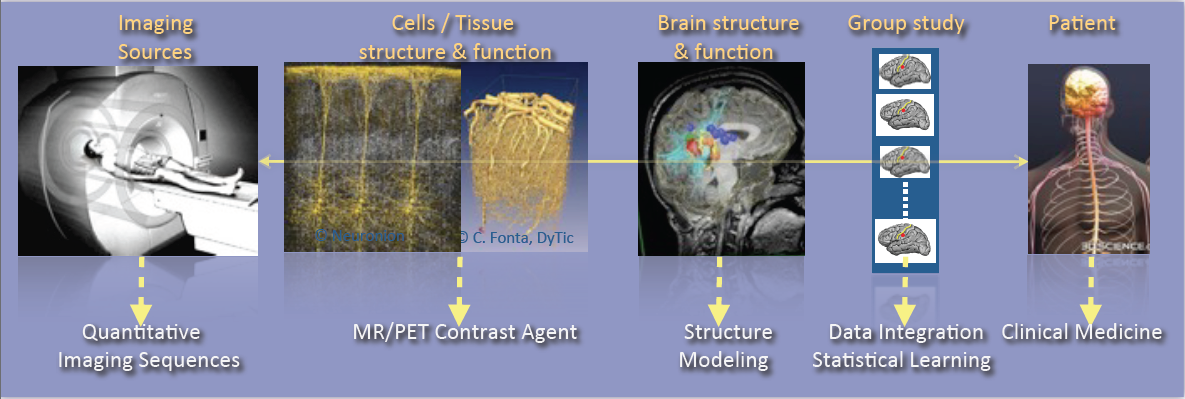
\includegraphics[width=\textwidth]{IMG/OverallObjectives}
          }
          \caption{
            The major overall scientific foundation of the team concerns the
            integration of data from the Imaging source to the patient at different
            scales: from the cellular or molecular level describing the structure and
            function, to the functional and structural level of brain structures and
            regions, to the population level for the modelling of group patterns and
            the learning of group or individual imaging markers.
          }
          \label{fig-objectives}
        \end{figure}
        
        As shown in Fig.~\ref{fig-objectives}, research activities of the
        \textsc{VisAGeS} U1228 team are tightly coupling observations and models through
        integration of clinical and multi-scale data, phenotypes (cellular, molecular
        or structural patterns). We work on personalized models of central nervous
        system organs and pathologies, and intend to confront these models to clinical
        investigation studies for quantitative diagnosis, prevention of diseases,
        therapy planning and validation. These approaches are developed in a
        translational framework where the data integration process to build the models
        inherits from specific clinical studies, and where the models are assessed on
        prospective clinical trials for diagnosis and therapy planning. All of this
        research activity is conducted in tight links with the
        \href{http://www.neurinfo.org}{Neurinfo} imaging platform environments and the
        engineering staff of the platform. In this context, some of our major
        challenges in this domain  concern:
        
        \begin{itemize}
          \item The elaboration of new descriptors to study the brain structure and
          function (e.g., variation of brain perfusion with and without contrast agent,
          evolution in shape and size of an anatomical structure in relation with
          normal, pathological or functional patterns, computation of asymmetries from
          shapes and volumes).
          \item The integration of additional spatio-temporal imaging sequences
          covering a larger range of observation, from the molecular level to the organ
          through the cell (Arterial Spin Labeling, diffusion MRI, MR relaxometry, MR
          cell labeling imaging, PET molecular imaging, …). This includes the
          elaboration of new image descriptors coming from spatio-temporal quantitative
          or contrast-enhanced MRI.
          \item The creation of computational models through data fusion of molecular,
          cellular, structural and functional image descriptors from group studies of
          normal and/or pathological subjects.
          \item The evaluation of these models on acute pathologies especially for the
          study of degenerative, psychiatric or developmental brain diseases (e.g.,
          Multiple Sclerosis, Epilepsy, Parkinson, Dementia, Strokes, Depression,
          Schizophrenia, …) in a translational framework.
        \end{itemize}
        
        In terms of methodological developments, we are particularly working on
        statistical methods for multidimensional image analysis, and feature selection
        and discovery, which include:
        
        \begin{itemize}
          \item The development of specific shape and appearance models, construction
          of atlases better adapted to a patient or a group of patients in order to
          better characterize the pathology;
          \item The development of advanced segmentation and modeling methods dealing
          with longitudinal and multidimensional data (vector or tensor fields),
          especially with the integration of new prior models to control the
          integration of multiscale data and aggregation of models;
          \item The development of new models and probabilistic methods to create water
          diffusion maps from MRI;
          \item The integration of machine learning procedures for classification and
          labeling of multidimensional features (from scalar to tensor fields and/or
          geometric features): pattern and rule inference and knowledge extraction are
          key techniques to help in the elaboration of knowledge in the complex domains
          we address;
          \item The development of new dimensionality reduction techniques for problems
          with massive data, which includes dictionary learning for sparse model
          discovery. Efficient techniques have still to be developed to properly
          extract from a raw mass of images derived data that are easier to analyze.
        \end{itemize}
        \end{module}



% \begin{module}{fondements}{test1}{LaTeX Test Page}

% %%% muni d'un titre, ce module apparaitra comme une sous-section

% Exemples d'équations :
  
% \begin{itemize}
% \item Equation en mode ``mathématique'' :\\

% $y=x^2$  

% \item Equation en environnement ``equation'' : \\

% \begin{equation}
%   P \left(\begin{array} {c}
%      \theta_{1} \\ \vdots  \\ \theta_{r}  
% \end{array}
%   \right) = Q + R, \label{noisident1}
% \end{equation}

% \item Equation en environnement ``displaymath'' : \\

% \begin{displaymath}
% \sum_{0}^{\infty} y = x^4
% \end{displaymath}

% \item Autre exemple :  

% \[ \forall f\in C^\infty\left(\left[-\frac{T}{2};\frac{T}{2}\right]\right),
%    \forall t\in \left[-\frac{T}{2};\frac{T}{2}\right],
%    f(\tau) = \sum_{k = -\infty}^{+\infty} e^{2i\pi\frac{k}{T}t} \times
%    \underbrace{\frac{1}{T}
%                \int_{-\frac{T}{2}}^{\frac{T}{2}} f(t) e^{-2i\pi\frac{k}{T}t} dt
%               }_{a_k = \tilde{f}\left(\nu = \frac{k}{T}\right)}
% \]

% \end{itemize}  

% Exemple de caractères spéciaux : \\  

% math pi : $\pi$ \\

% lettres : æ Æ à À â Â ä Ä ç Ç é É è È ê Ê ë Ë î Î ï Ï ô Ô ö Ö ù Ù û Û ü Ü ÿ {\th} {\TH}

% Exemples d'images :
  
% \begin{itemize}

% \item Image en jpeg : voir image \ref{fig:jpegimage} \\

% \begin{figure}
% \begin{center}
% 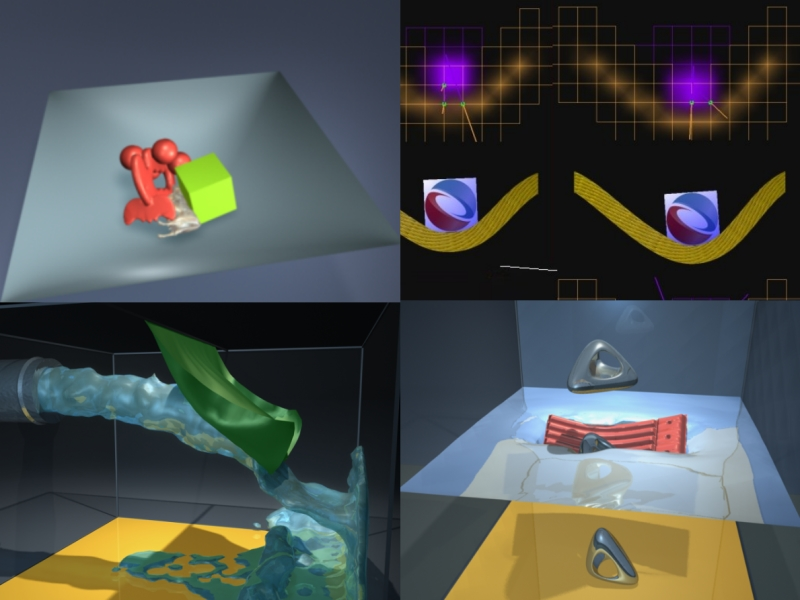
\includegraphics[width=4cm]{IMG/imagejpeg}
% \end{center}
% \caption{An example of a jpeg image}
% \label{fig:jpegimage}
% \end{figure}

% \item  Image en eps : voir figure \ref{fig:completemap} \\  

% \begin{figure}
% \begin{center}
% 
\includegraphics{IMG/imageeps}
% \end{center}
% \caption{An example of an eps file}
% \label{fig:completemap}
% \end{figure}

% \item Image en pdf : voir image \ref{fig:pdffile} \\  

% %\begin{center}
% \begin{figure}
% 
\includegraphics[width=2cm]{IMG/imagepdf}
% \caption{An example of a pdf file}
% \label{fig:pdffile}
% \end{figure}
% %\end{center}

% \end{itemize}

% \end{module}


%%% Un autre module dans la même section fondements  

% \begin{module}{fondements}{ident2}{Identification2}
% ...
% \end{module}


%%%%%%%%%%%%%%%%%%%%%%%%%%%%%%%%%%%%%%%%%%%%%%%%%%%%
%%%
%%% Section domaine (Application Domains)
%%% Il y a des modules ici
%%%
%%%%%%%%%%%%%%%%%%%%%%%%%%%%%%%%%%%%%%%%%%%%%%%%%%%%%

\begin{module}{domaine}{dom-neuro}{Neuroimaging}

One research objective in neuroimaging is the construction of anatomical and functional cerebral maps under normal and pathological conditions. Many researches are currently performed to find correlations between anatomical structures, essentially sulci and gyri, where neuronal activation takes place, and cerebral functions, as assessed by recordings obtained by the means of various neuroimaging modalities, such as PET (Positron Emission Tomography), fMRI (Functional Magnetic Resonance Imaging), EEG (Electro-EncephaloGraphy) and MEG (Magneto-EncephaloGraphy). Then, a central problem inherent to the formation of such maps is to put together recordings obtained from different modalities and from different subjects. This mapping can be greatly facilitated by the use of MR anatomical brain scans with high spatial resolution that allows a proper visualization of fine anatomical structures (sulci and gyri). Recent improvements in image processing techniques, such as segmentation, registration, delineation of the cortical ribbon, modeling of anatomical structures and multi-modality fusion, make possible this ambitious goal in neuroimaging. This problem is very rich in terms of applications since both clinical and neuroscience applications share similar problems. Since this domain is very generic by nature, our major contributions are directed towards clinical needs even though our work can address some specific aspects related to the neuroscience domain. 

\end{module}

\begin{module}{domaine}{dom-ms}{Multiple sclerosis}

Over the past years, a discrepancy became apparent between clinical Multiple sclerosis (MS) classification describing on the one hand MS according to four different disease courses and, on the other hand, the description of two different disease stages (an early inflammatory and a subsequently neurodegenerative phase). It is to be expected that neuroimaging will play a critical role to define in vivo those four different MS lesion patterns. An in vivo distinction between the four MS lesion patterns, and also between early and late stages of MS will have an important impact in the future for a better understanding of the natural history of MS and even more for the appropriate selection and monitoring of drug treatment in MS patients. MRI has a low specificity for defining in more detail the pathological changes which could discriminate between the different lesion types. However, it has a high sensitivity to detect focal and also widespread, diffuse pathology of the normal appearing white and gray matter. Our major objective within this application domain is then to define new neuroimaging markers for tracking the evolution of the pathology from high dimensional data (e.g., nD+t MRI) in the brain and the spinal cord. In addition, in order to complement MR neuroimaging data, we ambition to perform also cell labeling neuroimaging (e.g., MRI or PET) and to compare MR and PET data using standard and experimental MR contrast agents and radiolabeled PET tracers for activated microglia (e.g., USPIO or PK 11195). The goal is to define and develop, for routine purposes, cell specific and also quantitative imaging markers for the improved in vivo characterization of MS pathology. 

\end{module}

\begin{module}{domaine}{dom-anatfunc}{Modeling of anatomical and anatomo-functional neurological patterns}

The major objective within this application domain is to build anatomical and functional brain atlases in the context of functional mapping and for the study of developmental, neurodegenerative or even psychiatric brain diseases (Multiple sclerosis, Epilepsy, Parkinson, Dysphasia, Depression or even Alzheimer). This is a very competitive research domain; our contribution is based on our previous works in this field, and by continuing our local and wider collaborations. An additional objective within this application domain is to find new descriptors to study the brain anatomy and/or function (e.g., variation of brain perfusion, evolution in shape and size of an anatomical structure in relation with pathology or functional patterns, computation of asymmetries ...). This is also a very critical research domain, especially for many developmental or neurodegenerative brain diseases. 

\end{module}

%%%%%%%%%%%%%%%%%%%%%%%%%%%%%%%%%%%%%%%%%%%%%%%%%%%%%%%%%%%%%%%%%%%%%%%%%%%
%%%
%%% Section Highlights (Faits Marquants)
%%%  
%%% Les faits marquants doivent être relatifs aux résultats de l'année obtenus par votre équipe.
%%% L'obtention d'une HDR n'est pas un fait marquant.
%%% La sous-partie Awards (précédemment "Best papers") vous permet de signaler toute récompense, concernant une publication ou pas.  
%%% Tous types de publication récompensée peuvent être présentés ici. La récompense doit dater de l'année, la publication pas forcément.
%%% Citez-les dans la partie "Awards" sous la forme : \bestcite{xxxx}, \bestcite{yyyy}, ...  
%%%
%%% Documentation intranet : https://intranet.inria.fr/Vie-scientifique/Information-edition-scientifiques/RAweb/Les-sections#eztoc27554_8
%%%  
%%%
%%%%%%%%%%%%%%%%%%%%%%%%%%%%%%%%%%%%%%%%%%%%%%%%%%%%%%%%%%%%%%%%%%%%%%%%%%%%

\begin{module}{highlights}{NewHighlights}{}

\subsection{New reseracher}
Julie Coloigner was recruited as CNRS Researcher, starting from October 2018.

\subsection{New MRI at the Neurinfo platform}
A new 3T Siemens Prisma was installed at the Neuroinfo platform in February 2018. An official ceremony was organised with all the funders in November 2018.

\subsection{Award}
%% ICI vous pouvez ecrire du texte
%%
%% citez les "Awards" sous la forme : \bestcite{xxxx}, \bestcite{yyyy}, ...
Best poster award by the French Institute of Psychiatry for our communication at its annual Forum~\bestcite{coloigner:hal-01890087}.

\subsection{First neuroscience hackathon in Rennes}
We organised the first hackathon in the Visages team, April 25-26 as part of the international event Brainhack Global 2018.



\end{module}

%%%%%%%%%%%%%%%%%%%%%%%%%%%%%%%%%%%%%%%%%%%%%%%%%%%%%%%%%%%%%%%%%%%%%%%%%%%%%%
%%%
%%% Section logiciels et plateformes
%%%
%%%
%%% Information sur les données importées : logiciels
%%%  
%%% Il n'est pas possible de modifier le tex de la partie logiciel de cette section : les logiciels sont importés de la base BIL.  
%%% Il faut passer par BIL (https://bil.inria.fr/fr/catalog/listby/raweb) pour rajouter et compléter des logiciels.  
%%% Critères de sélection des logiciels pour le RA : avoir été développé ou avoir connu une évolution majeure ou importante en 2018.
%%% Le fichier tex du rapport est mis à jour automatiquement à chaque compilation.
%%% Il faut ensuite consulter le rapport en HTML et/ou en PDF pour vérifier le résultat.
%%%  
%%% Par contre la partie pour les platformes doit toujours être mise à jour manuellement à partir de ce fichier tex.
%%%
%%% Documentation intranet : https://intranet.inria.fr/Vie-scientifique/Information-edition-scientifiques/RAweb/Les-sections#eztoc27554_9
%%%
%%% En cas de problème : https://helpdesk.inria.fr/categories/181/submit
%%%
%%%%%%%%%%%%%%%%%%%%%%%%%%%%%%%%%%%%%%%%%%%%%%%%%%%%%%%%%%%%%%%%%%%%%%

%%%
%%% Ici la section logiciel va être incluse à la compilation    
%%% Il est possible de consulter le source tex qui va être inclus à l'adresse suivante :  
%%%     https://irabot.inria.fr/itramera?format=bil&epi=visages&annee=2018
%%%
%%%
%%% La partie Plaforms de la section logiciels et plateformes doit, le cas échéant, être complétée ici :  
%%%  

 \begin{module}{logiciels}{plateformexemple}{Platforms}  

\subsection{The Neurinfo Platform}

VisAGeS is the founding actor of an experimental research platform which was installed in August 2009 at the University Hospital of Rennes. The University of Rennes 1, Inria, Inserm for the academic side, and the University Hospital of Rennes and the Cancer Institute “Eugene Marquis” for the clinical side, are partners of this neuroinformatics platform called Neurinfo (http://www.neurinfo.org). This platform has been supported under the “Contrat de Projets Etat-Région” (Christian Barillot is the PI) and has received a total amount of 4.01 M€ for the period 2007–2014. European (FEDER), National (through Ministry of research, Inria, Inserm and ANR) and local councils (Brittany Region, Ille et Vilaine, and Rennes Metropole) have joined their effort to support this operation for a total amount of 4 010 k€ (600 k€ for the infrastructures, 2 850 k€ for the equipments and 560 k€ for the functioning). This application was set up through the Regional PIMATGI initiative coordinated by INSERM in Brittany (C. Roux). The overall PIMATGI initiative served for the financing of three distinct, but complementary, platforms: Neurinfo, TheraFONC as a technical platform dedicated to therapy guided by functional imaging especially in the oncology domain (Inserm U650 - LaTIM, Dir. Ch. Roux, Brest), and TherA-Image as a platform dedicated to image guided mini-invasive surgery and therapy especially in the domain of cardio-vascular diseases (U642 -LTSI, Dir. L. Senhadji, Rennes).

Concerning the Neurinfo Platform, the activity domain is a continuum between methodological and technological research built around specific clinical research projects. The ambition is to do innovation in science, technology and medical technology transfer for the implementation on the clinical field. On the medical field, the translational research domain mainly concerns medical imaging and more specifically the clinical neurosciences. Among them are multiple sclerosis, epilepsy, neurodegenerative, neurodevelopmental and psychiatric diseases, surgical procedures of brain lesions, neuro-oncology and radiotherapy planning. Beyond these CNS applications, the platform is also open to alternative applications. Neurinfo ambitions to support the emergence of research projects based on their level of innovation, their pluri-disciplinarity and their ability to foster collaborations between different actors (public and private research entities, different medical specialties, different scientific profiles).

In this context, a research 3T MRI system (Siemens Verio) was acquired in summer 2009 in order to develop the clinical research in the domain of morphological, functional, structural and cellular in-vivo imaging. In 2014 a new equipment for simultaneous recording of EEG and MRI images was acquired from Brain Product. In 2015, a mock scanner for experimental set-up was acquired as well as a new High Performance Computing environment made of one large computing cluster and a data center that is shared and operated by the Inria center at IRISA (UMR CNRS 6074). The computation cluster (240 cores) and the data center (up to 50 TB) are dedicated to host and process imaging data produced by the Neurinfo platform, but also by other research partners that share their protocols on the Neurinfo neuroinformatics system (currently more than 30 sites).

VisAGeS and its partners in the Neurinfo project are committed to use this new research platform for developing new regional, national and international collaborations around fundamental and applied clinical research projects dealing with in-vivo medical imaging.

In 2016, VisAGeS has been awarded by IBISA as a “Plateforme d'excellence”.

In 2017, funding was collected to replace the 3T Siemens Verio MRI that led to the installation of a new 3T Siemens Prisma in 2018.

 \end{module}


%%%%%%%%%%%%%%%%%%%%%%%%%%%%%%%%%%%%%%%%%%%%%%%%%%%%%%%
%%%
%%% Section Resultat nouveaux (New Results)
%%% Il y a des modules ici

%%%Documentation intranet : https://intranet.inria.fr/Vie-scientifique/Information-edition-scientifiques/RAweb/Les-sections#eztoc27554_10
%%%%%%%%%%%%%%%%%%%%%%%%%%%%%%%%%%%%%%%%%%%%%%%%%%%%%%%%

\begin{module}{resultats}{res-01}{Research axis 1: Medical Image Computing in Neuroimaging}
Extraction and exploitation of complex imaging biomarkers involve an imaging processing workflow that can be quite complex. This goes from image physics and image acquisition, image processing for quality control and enhancement, image analysis for features extraction and image fusion up to the final application which intends to demonstrate the capability of the image processing workflow to issue sensitive and specific markers of a given pathology. In this context, our objectives in the recent period were directed toward 4 major methodological topics:

\subsection{Diffusion imaging}

\subsubsection{Optimal selection of diffusion-weighting gradient waveforms using compressed sensing and dictionary learning}
\begin{participants}
      \pers{Raphaël}{Truffet}
      \pers{Emmanuel}{Caruyer}
\end{participants}
Acquisition sequences in diffusion MRI rely on the use time-dependent magnetic field gradients. Each gradient waveform encodes a diffusion weighted measure; a large number of such measurements are necessary for the in vivo reconstruction of microstructure parameters. We propose here a method to select only a subset of the measurements while being able to predict the unseen data using compressed sensing. We learn a dictionary using a training dataset generated with Monte-Carlo simulations; we then compare two different heuristics to select the measures to use for the prediction. We found that an undersampling strategy limiting the redundancy of the measures allows for a more accurate reconstruction when compared with random undersampling with similar sampling rate~\cite{truffet:inserm-01939066}.

\subsubsection{A Bayes Hilbert Space for Compartment Model Computing in Diffusion MRI}
\begin{participants}
      \pers{A.}{Stamm}
      \pers{O.}{Commowick}
      \pers{A.}{Menafoglio}
      \pers{S. K.}{Warfield}
\end{participants}
The single diffusion tensor model for mapping the brain white matter microstructure has long been criticized as providing sensitive yet non-specific clinical biomarkers for neurodegenerative diseases because (i) voxels in diffusion images actually contain more than one homogeneous tissue population and (ii) diffusion in a single homogeneous tissue can be non-Gaussian. Analytic models for compartmental diffusion signals have thus naturally emerged but there is surprisingly little for processing such images (estimation, smoothing, registration, atlas-ing, statistical analysis). We propose to embed these signals into a Bayes Hilbert space that we properly define and motivate. This provides a unified framework for compartment diffusion image computing. Experiments show that (i) interpolation in Bayes space features improved robustness to noise compared to the widely used log-Euclidean space for tensors and (ii) it is possible to trace complex key pathways such as the pyramidal tract using basic deterministic tractography thanks to the combined use of Bayes interpolation and multi-compartment diffusion models~\cite{stamm:inserm-01937992}

\subsubsection{Diffusion MRI as an imaging marker of depression from a large and homogenous population study}
\begin{participants}
      \pers{Julie}{Coloigner}
      \pers{Jean-Marie}{Batail}
      \pers{Isabelle}{Corouge}
      \pers{Jean-Christophe}{Ferre}
      \pers{Dominique}{Drapier}
      \pers{Christian}{Barillot}
\end{participants}
Despite the extensive therapy options available for depression, up to 80\% of patients will suffer from a relapse. Consequently, understanding the neural correlates underlying the depression will optimize the diagnosis and treatment of individual depressed patients. The purpose of our study was to investigate alterations of white matter integrity in a large cohort of patients suffering from depression using diffusion tensor imaging. Our findings provide robust evidence that the reduction of white-matter integrity in the interhemispheric connections and fronto-limbic neuronal circuits may play an important role in depression pathogenesis.~\cite{coloigner:hal-01812093}

\subsubsection{Diffusion MRI as a descriptive imaging marker of the pathogenesis of treatment-resistant depression}
\begin{participants}
      \pers{Julie}{Coloigner}
      \pers{Jean-Marie}{Batail}
      \pers{Isabelle}{Corouge}
      \pers{Jean-Christophe}{Ferre}
      \pers{Dominique}{Drapier}
      \pers{Christian}{Barillot}
\end{participants}
Despite the extensive therapy options available for depression, treatment-resistant depression (TRD) occurs in 20-30\% of depressed patients. Consequently, identification of neural changes in TRD could support to better understand the mechanism of resistance and to improve the treatment of individual depressed patients. We aimed to investigate the white-matter microstructure in a sample of depressed patients in which response to treatment was subsequently evaluated 6 months after. Our findings suggest the abnormalities of the white-matter integrity in multiple white matter tracts, such as anterior limb of internal capsule and genu of corpus may play a role in the pathogenesis of treatment-resistant depression.~\cite{coloigner:hal-01812087}

\subsubsection{White matter connectivity analysis in patients suffering from depression.
}
\begin{participants}
      \pers{Julie}{Coloigner}
      \pers{Jean-Marie}{Batail}
      \pers{Isabelle}{Corouge}
      \pers{Dominique}{Drapier}
      \pers{Christian}{Barillot}
\end{participants}
*TODO*~\cite{coloigner:hal-01890087}


\subsection{Arterial Spin Labeling}
\subsubsection{Patch-Based Super-Resolution of Arterial Spin Labeling Magnetic Resonance Images}
\begin{participants}
      \pers{Cédric}{Meurée}, 
      \pers{Pierre}{Maurel}, 
      \pers{Jean-Christophe}{Ferré},
      \pers{Christian}{Barillot}.
\end{participants}
Arterial spin labeling is a magnetic resonance perfusion imaging technique that, while providing results comparable to methods currently considered as more standard concerning the quantification of the cerebral blood flow, is subject to limitations related to its low signal-to-noise ratio and low resolution. In this work, we investigate the relevance of using a non-local patch-based super-resolution method driven by a high-resolution structural image to increase the level of details in arterial spin labeling images. This method is evaluated by comparison with other image dimension increasing techniques on a simulated dataset, on images of healthy subjects and on images of subjects diagnosed with brain tumors, who had a dynamic susceptibility contrast acquisition. The influence of an increase of ASL images resolution on partial volume effects is also investigated in this work.~\cite{meuree:inserm-01880726}

\subsubsection{Resting-state ASL : Toward an optimal sequence duration}
\begin{participants}
      \pers{Corentin}{Vallée}
      \pers{Pierre}{Maurel}, 
      \pers{Isabelle}{Corouge},
      \pers{Christian}{Barillot},
\end{participants}
Resting-state functional Arterial Spin Labeling (rs-fASL) in clinical daily practice and academic research stay discreet compared to resting-state BOLD. However, by giving direct access to cerebral blood flow maps, rs-fASL leads to significant clinical subject scaled application as CBF can be considered as a biomarker in common neuropathology. Our work here focuses on the link between overall quality of rs-fASL and duration of acquisition. To this end, we consider subject self-Default Mode Network (DMN), and assess DMN quality depletion compared to a gold standard DMN depending on the duration of acquisition~\cite{vallee:inserm-01935089}.


\subsection{Quantitative imaging}
%TODO: could also go in axis 2...
\subsubsection{Identification of Gadolinium contrast enhanced regions in MS lesions using brain tissue microstructure information obtained from diffusion and T2 relaxometry MRI}
\begin{participants}
      \pers{S.}{Chatterjee}
      \pers{O.}{Commowick}, 
      \pers{O.}{Afacan},
      \pers{S. K.}{Warfield},
      \pers{C.}{Barillot},
\end{participants}
A multiple sclerosis (MS) lesion at an early stage undergoes active blood brain barrier (BBB) breakdown. Identifying MS lesions in a patient which are undergoing active BBB breakdown is of critical importance for MS burden evaluation and treatment planning. However in non-contrast enhanced structural magnetic resonance imaging (MRI) the regions of the lesion undergoing active BBB breakdown cannot be distinguished from the other parts of the lesion. Hence gadolinium (Gd) contrast enhanced T1-weighted MR images are used for this task. However some side effects of Gd injection into patients have been increasingly reported recently. The BBB breakdown is reflected by the condition of tissue microstructure such as increased inflammation, presence of higher extra-cellular matter and debris. We thus propose a framework to predict enhancing regions in MS lesions using tissue microstructure information derived from T2 relaxometry and diffusion MRI (dMRI) multicompartment models. We show that combination of the dMRI and T2 relaxometry microstructure information can distinguish the Gd enhancing lesion regions from the other regions in MS lesions~\cite{chatterjee:hal-01830532}.


\subsubsection{Multi-Compartment Model of Brain Tissues from T2 Relaxometry MRI Using Gamma Distribution}
\begin{participants}
      \pers{S.}{Chatterjee}
      \pers{O.}{Commowick}, 
      \pers{O.}{Afacan},
      \pers{S. K.}{Warfield},
      \pers{C.}{Barillot},
\end{participants}
The brain microstructure, especially myelinated axons and free fluids, may provide useful insight into brain neurodegenerative diseases such as multiple sclerosis (MS). These may be distinguished based on their transverse relaxation times which can be measured using T2 relaxometry MRI. However, due to physical limitations on achievable resolution, each voxel contains a combination of these tissues, rendering the estimation complex. We present a novel multi-compartment T2 (MCT2) estimation based on variable projection, applicable to any MCT2 microstructure model. We derive this estimation for a three-gamma distribution model. We validate our framework on synthetic data and illustrate its potential on healthy volunteer and MS patient data~\cite{chatterjee:hal-01744852}.

% TODO: Could also go in axis 2
\subsubsection{A 3-year follow-up study of enhancing and non-enhancing multiple sclerosis (MS) lesions in MS patients demonstrating clinically isolated syndrome (CIS) using a multi-compartment T2 relaxometry (MCT2) model}
\begin{participants}
      \pers{S.}{Chatterjee}
      \pers{O.}{Commowick}, 
      \pers{O.}{Afacan},
      \pers{B.}{Combes},
      \pers{A.}{Kerbrat},
      \pers{S. K.}{Warfield},
      \pers{C.}{Barillot},
\end{participants}
Obtaining information on condition of tissue microstructures (such as myelin, intra/extra cellular cells, free water) can provide important insights into MS lesion. However, MRI voxels are heterogeneous in terms of tissue microstructure due to the limited imaging resolution owing to existing physical limitations of MRI scanners. Here we evaluated a multi-compartment T2 relaxometry model and then used it to study the evolution of enhancing (USPIO and gadolinium positive) and non-enhancing lesions in 6 MS patients with CIS characteristics over a period 3 years with 7 follow-up scans post baseline~\cite{chatterjee:hal-01821694}.

% TODO: Could also go in axis 2
\subsubsection{A three year follow-up study of gadolinium enhanced and non-enhanced regions in multiple sclerosis lesions using a multi-compartment T2 relaxometry model}
\begin{participants}
      \pers{S.}{Chatterjee}
      \pers{O.}{Commowick}, 
      \pers{O.}{Afacan},
      \pers{B.}{Combes},
      \pers{S. K.}{Warfield},
      \pers{C.}{Barillot},
\end{participants}
Demyelination, axonal damage and inflammation are critical indicators of the onset and progress of neurodegenerative diseases such as multiple sclerosis (MS) in patients. Due to physical limitations of imaging such as acquisition time and imaging resolution, a voxel in a MR image is heterogeneous in terms of tissue microstructure such as myelin, axons, intra and extra cellular fluids and free water. We present a multi-compartment tissue model which estimates the water fraction (WF) of tissues with short, medium and high T2 relaxation times in a T2 relaxometry MRI voxel. The proposed method is validated on test-retest data of healthy controls. This model was then used to study longitudinal trends of the tissue microstructures for two sub-regions of the lesions: gadolinium enhanced (E+) and non-enhanced (L−) regions of MS lesions in 10 MS patients over a period of three years. The water fraction values in E+ and L− regions were found to be significantly different (p < 0.05) over the period of first three months. The results of this study also showed that the estimates of the proposed T2 relaxometry model on brain tissue microstructures have potential to distinguish between regions undergoing active blood brain barrier breakdown from the other regions of the lesion~\cite{chatterjee:hal-01837974}.

\subsection{Atlases}
\subsubsection{Anisotropic similarity, a constrained affine transformation: Application to brain development analysis}
\begin{participants}
      \pers{A.}{Legouhy}
      \pers{O.}{Commowick}
      \pers{F.}{Rousseau}
      \pers{C.}{Barillot}
\end{participants}
The study of brain development provides insights in the normal trend of brain evolution and enables early detection of abnormalities. We propose a method to quantify brain growth in three arbitrary orthogonal directions of the brain through linear registration. We introduce a 9 degrees of freedom transformation that gives the opportunity to extract scaling factors describing brain growth along those directions by registering a database of subjects in a common basis. We apply this framework to create longitudinal curves of scaling ratios along fixed orthogonal directions from 0 to 16 years highlighting anisotropic brain development~\cite{legouhy:inserm-01871274}.


\subsection{Simultaneous EEG/fMRI}
\subsubsection{Automatic Electrodes Detection during simultaneous EEG/fMRI acquisition}
\begin{participants}
      \pers{M.}{Fleury}
      \pers{P.}{Maurel}
      \pers{M.}{Mano}
      \pers{E.}{Bannier}
      \pers{C.}{Barillot}
\end{participants}
Simultaneous EEG/fMRI acquisition allows to measure brain activity at high spatial-temporal resolution. The localisation ofEEG sources depends on several parameters including the position of the electrodes on the scalp. The position of the MRelectrodes during its acquisitions is obtained with the use of the UTE sequence allowing their visualisation. The retrieval ofthe electrodes consists in obtaining the volume where the electrodes are located by applying a sphere detectionalgorithm. We detect around 90\% of electrodes for each subject, and our UTE-based electrode detection showed anaverage position error of 3.7mm for all subjects~\cite{fleury:hal-01874815}.

\subsection{Inference in neuroimaging}
\subsubsection{Validity of summary statistics-based mixed-effects group fMRI}
\begin{participants}
      \pers{Camille}{Maumet}
      \pers{Thomas}{Nichols}
\end{participants}
Statistical analysis of multi-subject functional Magnetic Resonance Imaging (fMRI) data is traditionally done using either: 1) a mixed-effects GLM (MFX GLM) where within-subject variance estimates are used and incorporated into per-subject weights or 2) a random-effects General linear model (GLM) (RFX GLM) where within-subject variance estimates are not used. Both approaches are implemented and available in major neuroimaging software packages including: SPM (MFX analysis; 2nd-Level statistics), FSL (FLAME; OLS) and AFNI (3dMEMA; 3dttest++). While MFX GLM provides the most efficient statistical estimate, its properties are only guaranteed in large samples, and it has been shown that RFX GLM is a valid alternative for one-sample group analyses in fMRI [1]. We recently showed that MFX GLM for image-based meta-analysis could lead to invalid results in small-samples. Here, we investigate whether this issue also affects group fMRI~\cite{maumet:inserm-01887911}.

\subsubsection{Choosing a practical and valid Image-Based Meta-Analysis}
\begin{participants}
      \pers{Camille}{Maumet}
      \pers{Thomas}{Nichols}
\end{participants}
Meta-analysis provides a quantitative approach to summarise the rich functional Magnetic Resonance Imaging (fMRI) literature. When image data is available for each study, the optimal approach is to perform an Image-Based Meta-Analysis (IBMA) [1]. A number of IBMA approaches have been proposed including combination of standardised statistics (Z's), just effect estimates (E's) or both effect estimates and their standard errors (SE's). While using both E’s \& SE’s and estimating between-study variance should be optimal, the methods are not guaranteed to work for small number of studies. Also, often only standardised estimates are shared, reducing the possible meta-analytic approaches. Finally, because the BOLD signal is non-quantitative care has to be taken in order to insure that E's are expressed in the same units [2,3], especially when combining data from different software packages. Given the growing interest in data sharing in the neuroimaging community there is a need to identify what is the minimal data to be shared in order to allow for future IBMAs. Here, we investigate the validity of 8 IBMA approaches~\cite{maumet:inserm-01933032}.

\end{module}


\begin{module}{resultats}{res-02}{Research axis 2: Applications in Neuroradiology and Neurological Disorders}

\subsection{Bimodal EEG-fMRI Neurofeedback for Stroke Rehabilitation: a Case Report}
\begin{participants}
      \pers{Giulia}{Lioi}, 
      \pers{Mathis}{Fleury}, 
      \pers{Simon}{Butet},
      \pers{Anatole}{Lécuyer},
      \pers{Christian}{Barillot},
      \pers{Isabelle}{Bonan}.
\end{participants}
Neurofeedback  (NF)  consists  on  training  self-regulation  of  brain  activity  by  providing  real-time information about the participant brain function.  Few works have shown the potential of NF for stroke rehabilitation however its effectiveness has not been investigated yet. NF approaches are usually based on real-time monitoring of brain activity using a single imaging technique.  Recent studies have revealed the potential of combining EEG and fMRI to achieve a more efficient and specific self-regulation. In this case report, we tested the feasibility of applying bimodal EEG-MRI NF on two stroke patients.~\cite{lioi:inserm-01932954}

% TODO: Could also go in 3
\subsection{Statistical Shape Analysis of Large Datasets Based on Diffeomorphic Iterative Centroids}
\begin{participants}
      \pers{C.}{Cury}
      \pers{J.}{Glaunès}, 
      \pers{R.}{Toro},
      \pers{M.}{Chupin},
      \pers{G.}{Schumann},
      \pers{V.}{Frouin},
      \pers{J.-B.}{Poline},
      \pers{O.}{Colliot},
\end{participants}
In this paper, we propose an approach for template-based shape analysis of large datasets, using diffeomorphic centroids as atlas shapes. Diffeomorphic centroid methods fit in the Large Deformation Diffeomorphic Metric Mapping (LDDMM) framework and use kernel metrics on currents to quantify surface dissimilarities. The statistical analysis is based on a Kernel Principal Component Analysis (Kernel PCA) performed on the set of initial momentum vectors which parametrize the deformations. We tested the approach on different datasets of hippocampal shapes extracted from brain magnetic resonance imaging (MRI), compared three different centroid methods and a variational template estimation. The largest dataset is composed of 1,000 surfaces, and we are able to analyse this dataset in 26 h using a diffeomorphic centroid. Our experiments demonstrate that computing diffeomorphic centroids in place of standard variational templates leads to similar shape analysis results and saves around 70\% of computation time. Furthermore, the approach is able to adequately capture the variability of hippocampal shapes with a reasonable number of dimensions, and to predict anatomical features of the hippocampus, only present in 17\% of the population, in healthy subjects.~\cite{cury:hal-01920263}.


\subsection{Refining understanding of working memory buffers through the construct of binding: Evidence from a single case informs theory and clinical practise}
\begin{participants}
      \pers{Pierre-Yves}{Jonin}
      \pers{Clara}{Calia}, 
      \pers{Sophie}{Muratot},
      \pers{Serge}{Belliard},
      \pers{Quentin}{Duché},
      \pers{Emmanuel}{Barbeau},
      \pers{Mario.}{Parra},
\end{participants}
Binding operations carried out in working memory enable the integration of information from different sources during online performance. While available evidence suggests that working memory may involve distinct binding functions, whether or not they all involve the episodic buffer as a cognitive substrate remains unclear. Similarly, knowledge about the neural underpinnings of working memory buffers is limited, more specifically regarding the involvement of medial temporal lobe structures. In the present study, we report on the case of patient KA, with developmental amnesia and selective damage to the whole hippocampal system. We found that KA was unable to hold shape-colours associations (relational binding) in working memory. In contrast, he could hold integrated coloured shapes (conjunctive binding) in two different tasks. Otherwise, and as expected, KA was impaired on three relational memory tasks thought to depend on the hippocampus that are widely used in the early detection of Alzheimer's disease. Our results emphasize a dissociation between two binding processes within working memory, suggesting that the visuo-spatial sketchpad could support conjunctive binding, and may rely upon a large cortical network including sub-hippocampal structures. By contrast, we found evidence for a selective impairment of relational binding in working memory when the hippocampal system is compromised, suggesting that the long-term memory deficit observed in amnesic patients may be related to impaired short-term relational binding at encoding. Finally, these findings may inform research on the early detection of Alzheimer's disease as the preservation of conjunctive binding in KA is in sharp contrast with the impaired performance demonstrated very early in this disease.
.~\cite{jonin:inserm-01916090}.

\subsection{Superior explicit memory despite severe developmental amnesia: In-depth case study and neural correlates}
\begin{participants}
      \pers{Pierre-Yves}{Jonin}
      \pers{Gabriel}{Besson}, 
      \pers{Renaud}{La Joie},
      \pers{Jérémie}{Pariente},
      \pers{Serge}{Belliard},
      \pers{Christian}{Barillot},
      \pers{Emmanuel}{Barbeau},
\end{participants}
The acquisition of new semantic memories is sometimes preserved in patients with hippocampal amnesia. Robust evidence for this comes from case reports of developmental amnesia suggesting that low-to-normal levels of semantic knowledge can be achieved despite compromised epi-sodic learning. However, it is unclear whether this relative preservation of semantic memory results from normal acquisition and retrieval or from residual episodic memory, combined with effortful repetition. Furthermore, lesion studies have mainly focused on the hippocampus itself, and have seldom reported the state of structures in the extended hippocampal system. Preserved components of this system may therefore mediate residual episodic abilities, contributing to the apparent semantic preservation. We report an in-depth study of Patient KA, a 27-year-old man who had severe hypoxia at birth, in which we carefully explored his residual episodic learning abilities. We used novel speeded recognition paradigms to assess whether KA could explicitly acquire and retrieve new context-free memories. Despite a pattern of very severe amnesia, with a 44-point discrepancy between his intelligence and memory quotients, KA exhibited normal-to-superior levels of knowledge, even under strict time constraints. He also exhibited normal-to-superior recognition memory for new material, again under strict time constraints. Mul-timodal neuroimaging revealed an unusual pattern of selective atrophy within each component of the extended hippocampal system, contrasting with the preservation of anterior subhippocampal cortices. A cortical thickness analysis yielded a pattern of thinner but also thicker regional cortices, pointing toward specific temporal lobe reorganization following early injury. We thus report the first case of superior explicit learning and memory in a severe case of amnesia, raising important questions about how such knowledge can be acquired~\cite{jonin:inserm-01916086}.


\subsection{Retrieval practice based on recognition memory: testing the retrieval effort hypothesis}
\begin{participants}
      \pers{Pierre-Yves}{Jonin}
      \pers{Audrey}{Noël}, 
      \pers{Gabriel}{Besson},
      \pers{Sophie}{Muratot},
      \pers{Serge}{Belliard},
      \pers{Christian}{Barillot},
      \pers{Emmanuel}{Barbeau},
\end{participants}
We tested a core prediction of the retrieval effort hypothesis as an account for the testing effect (TE). Retrieval effort predicts that automatic, effortful retrieval should not lead to TE. Experiment 1 (N=76) showed that despite an encoding duration of three times less, object pictures retention is better after repeated testing under Old/New recognition conditions, than following repeated study. Experiment 2 (N=30) used a speeded and accuracy boosting procedure to rule out the contribution of recollection to retrieval. Retention of object pictures at 25 minutes and 6 months was similar after repeated testing or after repeated studying. These results call for a revision of the retrieval effort hypothesis as a mechanistic account of TE~\cite{jonin:inserm-01939069}.


\subsection{Voxel-wise Comparison with a-contrario Analysis for Automated Segmentation of Multiple Sclerosis Lesions from Multimodal MRI}
\begin{participants}
      \pers{Francesca}{Galassi}
      \pers{Olivier}{Commowick},
      \pers{Emmanuel}{Vallee},
      \pers{Christian}{Barillot},
\end{participants}
We introduce a new framework for the automated and un-supervised segmentation of Multiple Sclerosis lesions from multimodal Magnetic Resonance images. It relies on a voxel-wise approach to detect local white matter abnormalities, with an a-contrario analysis, which takes into account local information. First, a voxel-wise comparison of multimodal patient images to a set of controls is performed. Then, region-based probabilities are estimated using an a-contrario approach. Finally, correction for multiple testing is performed. Validation was undertaken on a multi-site clinical dataset of 53 MS patients with various number and volume of lesions. We showed that the proposed framework outperforms the widely used FDR-correction for this type of analysis, particularly for low lesion loads~\cite{galassi:inserm-01888928}.

\subsection{Integration of Probabilistic Atlas and Graph Cuts for Automated Segmentation of Multiple Sclerosis lesions}
\begin{participants}
      \pers{Francesca}{Galassi}
      \pers{Olivier}{Commowick},
      \pers{Christian}{Barillot},
\end{participants}
We propose a framework for automated segmentation of Multiple Sclerosis (MS) lesions
from MR brain images. It integrates a priori tissues and MS lesions information into a Graph-Cuts algorithm for improved segmentation results.~\cite{galassi:hal-01823801}.

\subsection{Multiple sclerosis}
\begin{participants}
      \pers{Anne}{Kerbrat}
      \pers{Gilles}{Edan}
      \pers{Jean-Christophe}{Ferré}
      \pers{Benoit}{Combès}
      \pers{Olivier}{Commowick}
      \pers{Élise}{Bannier}
      \pers{Sudhanya}{Chatterjee}
      \pers{Haykel}{Snoussi}
      \pers{Emmanuel}{Caruyer}
      \pers{Christian}{Barillot}
\end{participants}
The VisAGeS research team has a strong focus on applying the developed methodologies (illustrated in research axis 1) to multiple sclerosis (MS) understanding and the prediction of its evolution. Related to the EMISEP project on spinal cord injury evolution in MS, a first work investigated the magnetization transfer reproducibility across centers in the spinal cord and was accepted for publication (JMRI 2018). Based on this work, a second work investigated the sensitivity of magnetization transfer to assess diffuse and focal burden in MS patients and was published in Mult. Sclerosis. 


\end{module}

\begin{module}{resultats}{res-03}{Research axis 3: Management of Information in Neuroimaging}

% TODO: olivier proposait en 1 ou 2
\subsection{Objective Evaluation of Multiple Sclerosis Lesion Segmentation using a Data Management and Processing Infrastructure}
\begin{participants}
      \pers{O.}{Commowick},
      \pers{A.}{Istace},
      \pers{M.}{Kain},
      \pers{B.}{Laurent},
      \pers{F.}{Leray},
      \pers{M.}{Simon},
      \pers{S. C.}{Pop},
      \pers{P.}{Girard},
      \pers{R.}{Ameli},
      \pers{J.-C.}{Ferré},
      \pers{A.}{Kerbrat},
      \pers{T.}{Tourdias},
      \pers{F.}{Cervenansky},
      \pers{T.}{Glatard},
      \pers{J.}{Beaumont},
      \pers{S.}{Doyle},
      \pers{F.}{Forbes},
      \pers{J.}{Knight},
      \pers{A.}{Khademi},
      \pers{A.}{Mahbod},
      \pers{C.}{Wang},
      \pers{R.}{Mckinley},
      \pers{F.}{Wagner},
      \pers{J.}{Muschelli},
      \pers{E.}{Sweeney},
      \pers{E.}{Roura},
      \pers{X.}{Lladó},
      \pers{M. M.}{Santos},
      \pers{W. P.}{Santos},
      \pers{A. G.}{Silva-Filho},
      \pers{X.}{Tomas-Fernandez},
      \pers{H.}{Urien},
      \pers{I.}{Bloch},
      \pers{S.}{Valverde}
      \pers{M.}{Cabezas},
      \pers{F. J.}{Vera-Olmos},
      \pers{N.}{Malpica},
      \pers{C. R. G.}{Guttmann},
      \pers{S.}{Vukusic},
      \pers{G.}{Edan},
      \pers{M.}{Dojat},
      \pers{M.}{Styner},
      \pers{S. K.}{Warfield},
      \pers{F.}{Cotton},
      \pers{C.}{Barillot}
\end{participants}
We present a study of multiple sclerosis segmentation algorithms conducted at the international MICCAI 2016 challenge. This challenge was operated using a new open-science computing infrastructure. This allowed for the automatic and independent evaluation of a large range of algorithms in a fair and completely automatic manner. This computing infrastructure was used to evaluate thirteen methods of MS lesions segmentation, exploring a broad range of state-of-the-art algorithms, against a high-quality database of 53 MS cases coming from four centers following a common definition of the acquisition protocol. Each case was annotated manually by an unprecedented number of seven different experts. Results of the challenge highlighted that automatic algorithms, including the recent machine learning methods (random forests, deep learning,...), are still trailing human expertise on both detection and delineation criteria. In addition, we demonstrate that computing a statistically robust consensus of the algorithms performs closer to human expertise on one score (segmentation) although still trailing on detection scores~\cite{commowick:inserm-01847873}

\subsection{Open Science for the Neuroinformatics community}
\begin{participants}
      \pers{Sorina}{Pop}
      \pers{Axel}{Bonnet}
      \pers{Camille}{Maumet}
      \pers{Michael}{Kain}
      \pers{Christian}{Barillot}
      \pers{Tristan}{Glatard}
\end{participants}
The Neuroinformatics community in OpenAire-Connect is represented by members of the France Life Imaging (FLI) collaboration. In this context, we aim at leveraging OpenAire-Connect services and give our community members the possibility to easily publish and exchange research artefacts from FLI platforms, such as VIP and Shanoir. This will enable open and reproducible science, since literature, data, and methods can be linked, retrieved, and replayed by all the members of the community~\cite{pop:inserm-01846994}.

\subsection{Interoperability with Boutiques and CARMIN}
\begin{participants}
      \pers{Sorina}{Pop}
      \pers{Axel}{Bonnet}
      \pers{Camille}{Maumet}
      \pers{Michael}{Kain}
      \pers{Christian}{Barillot}
      \pers{Tristan}{Glatard}
\end{participants}
A growing number of platforms and tools have lately been developed to meet the needs of various scientific communities. Most of these solutions are optimized to specific requirements from different user groups, leading to technological fragmentation and lack of interoperability. In our quest of open and reproducible science, we propose two complementary tools, Boutiques and CARMIN, providing cross-platform interoperability for scientific applications, data sharing and processing~\cite{pop:inserm-01846997}.

\subsection{A standardised representation for non-parametric fMRI results}
\begin{participants}
      \pers{Camille}{Maumet}
      \pers{Guillaume}{Flandin},
      \pers{Martin}{Perez-Guevara},
      \pers{Jean-Baptiste}{Poline},
      \pers{Justin}{Rajendra},
      \pers{Richard}{Reynolds},
      \pers{Bertrand}{Thirion},
      \pers{Thomas}{Nichols}
\end{participants}
Reuse of data collected and analysed at another site is becoming more prevalent in the neuroimaging community (cf. for example (Milham et al. 2017)) but this process usually relies on intensive data and metadata curation. Given the ever-increasing number of research datasets produced and shared, it is desirable to rely on standards that will enable automatic data and metadata retrieval for large-scale analyses (Wilkinson et al. 2016). We recently introduced NIDM-Results (Maumet et al. 2016), a data model to represent and publish data and metadata created as part of a mass univariate neuroimaging study (typically functional magnetic resonance imaging). Here we extend this model to allow for the representation of non-parametric analyses and we introduce a JSON API that will facilitate export into NIDM-Results~\cite{maumet:inserm-01828914}.

\subsection{Development of an Ontology for the INCF Neuroimaging Data Model (NIDM)}
\begin{participants}
      \pers{K. G.}{Helmer}, 
      \pers{K. B.}{David}, 
      \pers{T.}{Auer}, 
      \pers{S.}{Ghosh}, 
      \pers{C.}{Maumet},
      \pers{T. E.}{Nichols}, 
      \pers{P.}{Smruti},
      \pers{J.-B.}{Poline}
\end{participants}
The successful reuse of shared data relies on the existence of easily-available well-described metadata [1]. The metadata, as a rich description of the data, must capture information on how the data was acquired, processed and analyzed. The terms used to describe the data should be chosen with a logical, consistent framework in mind and include definitions to avoid ambiguity. In addition, a lexicon or ontology should reuse terms from existing efforts as much as possible [2]~\cite{helmer:inserm-01932994}.

\subsection{Same Data - Different Software - Different Results? Analytic Variability of Group fMRI Results}
\begin{participants}
      \pers{Alexander}{Bowring}
      \pers{Camille}{Maumet}
      \pers{Thomas}{Nichols}
\end{participants}
A wealth of analysis tools are available to fMRI researchers in order to extract patterns of task variation and, ultimately, understand cognitive function. However, this 'methodological plurality' comes with a drawback. While conceptually similar, two different analysis pipelines applied on the same dataset may not produce the same scientific results. Differences in methods, implementations across software packages, and even operating systems or software versions all contribute to this variability. Consequently, attention in the field has recently been directed to reproducibility and data sharing. Neuroimaging is currently experiencing a surge in initiatives to improve research practices and ensure that all conclusions inferred from an fMRI study are replicable. In this work, our goal is to understand how choice of software package impacts on analysis results. We use publically shared data from three published task fMRI neuroimaging studies, reanalyzing each study using the three main neuroimaging software packages, AFNI, FSL and SPM, using parametric and nonparametric inference. We obtain all information on how to process, analyze, and model each dataset from the publications. We make quantitative and qualitative comparisons between our replications to gauge the scale of variability in our results and assess the fundamental differences between each software package. While qualitatively we find broad similarities between packages, we also discover marked differences, such as Dice similarity coefficients ranging from 0.000-0.743 in comparisons of thresholded statistic maps between software. We discuss the challenges involved in trying to reanalyse the published studies, and highlight our own efforts to make this research reproducible~\cite{bowring:inserm-01933019,bowring:inserm-01760535}.

\subsection{Detecting and Interpreting Heterogeneity and Publication Bias in Image-Based Meta-Analyses}
\begin{participants}
      \pers{Thomas}{Maullin-Sapey}
      \pers{Camille}{Maumet}
      \pers{Thomas}{Nichols}
\end{participants}
With the increase of data sharing, meta-analyses are becoming increasingly important in the neuroimaging community. They provide a quantitative summary of published results and heightened confidence due to higher statistical power. The gold standard approach to combine results from neuroimaging studies is an Image-Based Meta-Analysis (IBMA) [1] in which group-level maps from different studies are combined. Recently, we have introduced the IBMA toolbox, an extension for SPM that provides methods for combining image maps from multiple studies [2]. However, the current toolbox lacks diagnostic tools used to assess critical assumptions of meta-analysis, in particular whether there is inter-study variation requiring random-effects IBMA, and whether publication bias is present. Here, we present two new tools added to the IBMA toolbox to detect heterogeneity and to assess evidence of publication bias~\cite{maullinsapey:inserm-01933023}.

\end{module}

%%\begin{module}{resultats}{new2}{New result 2}
%%ICI Vous pouvez ecrire du texte
%%\end{module}



%%%%%%%%%%%%%%%%%%%%%%%%%%%%%%%%%%%%%%%%%%%%%%%%%%%%%%%
%%%
%%% Section contrats (Bilateral Contracts and Grants with Industry)
%%% Il y a des modules ici
%%%
%%% Documentation intranet : https://intranet.inria.fr/Vie-scientifique/Information-edition-scientifiques/Comment-rediger-le-RAweb/Les-sections#eztoc27554_11
%%%%%%%%%%%%%%%%%%%%%%%%%%%%%%%%%%%%%%%%%%%%%%%%%%%%%%%


\begin{module}{contrats}{cgwi1}{Bilateral Contracts with Industry}

\subsection{Siemens}
In the context of the Neurinfo imaging platform, a master research agreement between Siemens SAS - Healthcare and University of Rennes 1 defines the terms of the collaboration between Siemens, Visages and the Neurinfo platform. Relying on
this research agreement contract, Neurinfo has received work in progress (WIP) sequences from Siemens in the form of object code for evaluation in the context of clinical research. The Neurinfo platform has also received source code of selected MRI sequences. As an example, the diffusion sequence code was modified to load arbitrary diffusion gradient waveforms for the FastMicroDiff project led by E. Caruyer. This is crucial in the collaboration since it enables the development of MRI sequences on site. Siemens currently provides research resources through the funding of a PhD student (Cédric Meurée: CIFRE Inria / Siemens grant). The MR Diffusion pulse sequence source code was modified in collaboration with our Siemens clinical scientist as part of our Master Research Agreement, Marc Lapert, in order to play arbitrary gradient waveforms. This was done on the Syngo VB17 software version and again on VE11C (nearly finished).

\end{module}

\begin{module}{contrats}{cgwi2}{Bilateral Grants with Industry}
The PhD of Cédric Meurée is funded by Siemens Healthineers under a CIFRE grant. 
\end{module}


%%%%%%%%%%%%%%%%%%%%%%%%%%%%%%%%%%%%%%%%%%%%%%%%%%%%%%%%%%%%%%%%%
%%%
%%% Section partenariat (Partnerships and Cooperations)
%%% Il y a des modules ici
%%%
%%% Dans cette section, certains modules sont **normalises**.
%%% Par consequent, la liste de ces modules
%%% est :
%%%  
%%% \begin{module}{partenariat}{regional}{Regional Initiatives}
%%% \begin{module}{partenariat}{national}{National Initiatives}
%%% \begin{module}{partenariat}{europe}{European Initiatives}
%%% \begin{module}{partenariat}{international}{International Initiatives}
%%% \begin{module}{partenariat}{visites}{International Research Visitors}
%%%  
%%% On peut, en outre, ajouter des modules pour insérer ce qui ne  
%%% rentre pas dans les catégories ci-dessus. Pour chacun des modules  
%%% listés, les actions proprement dites apparaitront en  
%%% \subsubsection, et les listes de {participants} seront ventilées en  
%%% conséquence, par \subsubsection (et non plus par module)
%%%  
%%% Documentation intranet : https://intranet.inria.fr/Vie-scientifique/Information-edition-scientifiques/Comment-rediger-le-RAweb/Les-sections#eztoc27554_12
%%%%%%%%%%%%%%%%%%%%%%%%%%%%%%%%%%%%%%%%%%%%%%%%%%%%%%%%%%%%%%%%%%%

\begin{module}{partenariat}{regional}{Regional Initiatives}
%% ICI Vous pouvez ecrire du texte

\subsection{INCR: MUltiple Sclerosis Imaging Check-out (MUSIC)}
    \begin{participants}
      \pers{Gilles}{Edan}
      \pers{Francesca}{Galassi}
      \pers{Olivier}{Commowick}
      \pers{Christian}{Barillot}
      \pers{Anne}{Kerbrat}
      \pers{Jean-Christophe}{Ferre}
    \end{participants}
The objective of this project is to investigate algorithms aimed at detecting, segmenting and following overtime the MS lesions, robustly enough to work on a multi-site clinical database. Methods are being evaluated on an amount of training and testing MS images with high quality segmentations from radiographers.
The goal is to integrate the developed framework into a production workflow that will be employed by the clinical health network MUltiple Sclerosis Imaging Check-out (MUSIC), covering the western part of France.

\end{module}


\begin{module}{partenariat}{national}{National Initiatives}

        \subsection{Projet Fondation de France: PERINE}
    \begin{participants}
      \pers{Élise}{Bannier}, 
      \pers{Isabelle}{Corouge}, 
      \pers{Julie}{Coloigner}, 
      \pers{Maia}{Proisy}, 
      \pers{Jean-Christophe}{Ferré},
      \pers{Christian}{Barillot}.
    \end{participants}
    This study evaluates the effect of prenatal exposure to neurotoxicants on the
    developing brain. Following previous studies in the PELAGIE cohort this MRI
    study involves ASL, Diffusion and working memory as well as motor inhibition
    BOLD fMRI together with neuropsychological tests in children. Inclusions have
    started in November 2014 and lasted for 2 years.  The MRI acquisitions of the
    PERINE projects have all been performed and 101 children included. A PhD started in January 2017 to process the functional MRI data of this
    project and Julie Coloigner was hired as a post doc to work on the Diffusion and ASL data.
    
    \subsection{Projet Fondation de France: EPMR-MA}
    \begin{participants}
      \pers{Pierre-Yves}{Jonin},
      \pers{Élise}{Bannier}, 
      \pers{Christian}{Barillot}, 
      \pers{Quentin}{Duché}, 
    \end{participants}
    This project evaluates memory effects in healthy adults and in patients
    presenting cognitive impairments using BOLD fMRI and diffusion MRI. 
    The inclusions of patients started in 2016 and all inclusions will be over by the end of 2017. Quentin Duché was hired to process the functional MRI and diffusion data end of 2016 and his contract was extended until May 2018. 
       
        \subsection{ANR "MAIA", 2015 generic projects program}
        \label{sssec:anr_maia}
        \begin{participants}
          \pers{Maia}{Proisy}
          \pers{Pierre}{Maurel}
          \pers{Antoine}{Legouhy}
          \pers{Olivier}{Commowick}
          \pers{Isabelle}{Corouge}
          \pers{Jean-Christophe}{Ferré}
          \pers{Christian}{Barillot}
        \end{participants}
        Each year in France, 55 000 children are born prematurely, i.e., before the
        37th week of gestation. Long-term studies of the outcome of prematurely born
        infants have clearly documented that the majority of such infants may have
        significant motor, cognitive, and behavioral deficits.
        
        However, there is a limited understanding of the nature of the cerebral
        abnormality underlying these adverse neurologic outcomes.  In this context, the
        emergence of new modalities of 3D functional MRI, e.g., Arterial Spin Labeling
        (ASL), or optical imaging technologies, e.g., Near InfraRed Spectroscopy
        (NIRS), brings new perspectives for extracting cognitive information, via
        metabolic activity measures. Other classical techniques devoted to cerebral
        signal measurement, such as ElectroEncephaloGraphy (EEG), provide cognitive
        information at the cortical level. Each of these various non-invasive imaging
        technologies brings substantial and specific information for the understanding
        of newborn brain development.
        
        This project aims at developing innovative approaches for multi-image /
        multi-signal analysis, in order to improve neurodevelopment understanding
        methods. From a fundamental point of view, mathematics and computer science
        have to be considered in association with imaging physics and medicine, to deal
        with open issues of signal and image analysis from heterogeneous data (image,
        signal), considered in the multiphysics contexts related to data acquisition
        (magnetic, optic, electric signals) and biophysics modeling of the newborn
        brain. A sustained synergy between all these scientific domains is then
        necessary.
        
        Finally, the sine qua non condition to reach a better understanding of the
        coupled morphological- cognitive development of premature newborns, is the
        development of effective software tools, and their distribution to the whole
        medical community. The very target of this project will be the design of such
        software tools for medical image / signal analysis, actually operational in
        clinical routine, and freely available. Academic researchers and industrial
        partners will work in close collaboration to reach that ambitious goal.


        \begin{figure}[htbp]
          \centerline{
            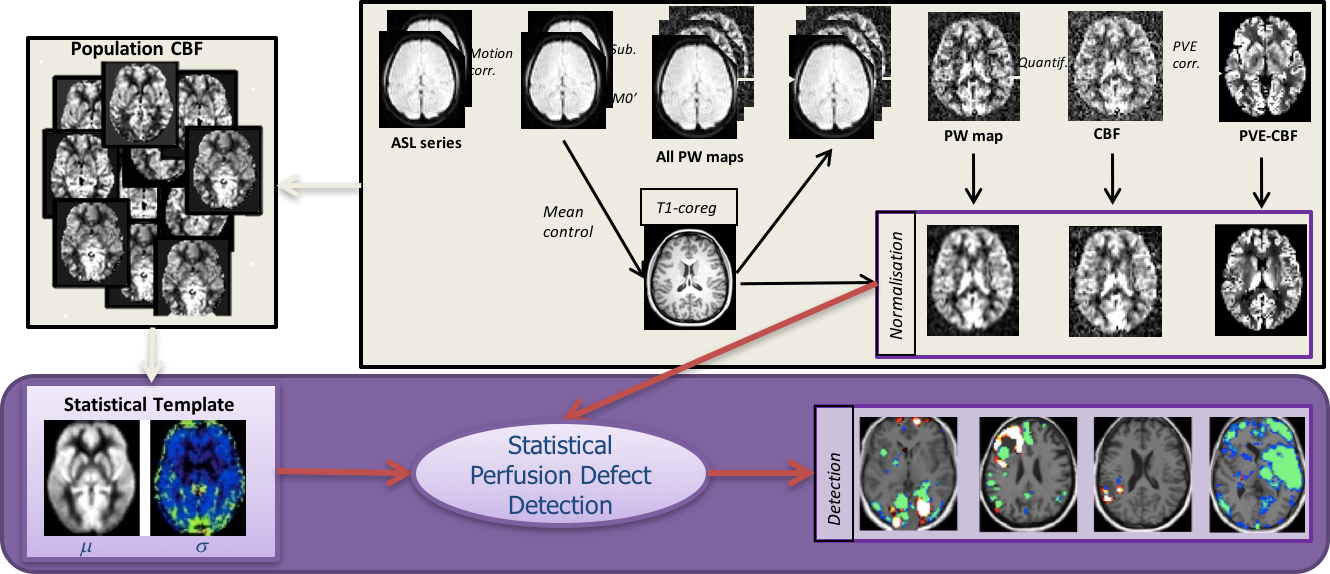
\includegraphics[width=\textwidth]{IMG/ASL_quantification}
          }
        \end{figure}
        
         \subsection{Fondation pour la recherche médicale (FRM) - Project "Hybrid EEG/IRM Neurofeedback for  rehabilitation of brain pathologies}
        \begin{participants}
        	\pers{Élise}{Bannier}, 
        	\pers{Jean-Marie}{Batail},
        	\pers{Isabelle}{Bonan}, 
        	\pers{Isabelle}{Corouge},
        	\pers{Jean-Christophe}{Ferré}, 
        	\pers{Jean-Yves}{Gauvrit}, 
        	\pers{Pierre}{Maurel}, 
        	\pers{Mathis}{Fleury},
        	\pers{Giulia}{Lioi}, 
        	\pers{Christian}{Barillot}
        \end{participants}	
        
        The goal of this project is to make full use of neurofeedback (NF) paradigm in the context of brain
rehabilitation. The major breakthrough will come from the coupling associating functional and
metabolic information from Magnetic Resonance Imaging (fMRI) to Electro-encephalography (EEG)
to “optimize” the neurofeedback protocol. We propose to combine advanced instrumental devices
(Hybrid EEG and MRI platforms), with new hybrid Brain computer interface (BCI) paradigms and
new computational models to provide novel therapeutic and neuro-rehabilitation paradigms in
some of the major mental and neurological disorders of the developmental and the aging brain
(stroke, language disorders, Mood Depressive Disorder (MDD), …). Though the concept of using
neurofeedback paradigms for brain therapy has somehow been experimented recently (mostly
through case studies), performing neurofeedback through simultaneous fMRI and EEG has almost
never been done before so far (two teams in the world including us within the HEMISFER CominLabs project).
This project will be conducted through a very complementary set of competences over the different
involved teams: VISAGES U1228, HYBRID and PANAMA Teams from Inria/Irisa Rennes and EA 4712
team from U. of Rennes I.

  \subsection{PHRC EMISEP: Evaluation of early spinal cord injury and late
	physical disability in Relapsing Remitting Multiple Sclerosis}
\begin{participants}
	\pers{Élise}{Bannier}, 
	\pers{Christian}{Barillot},
	\pers{Emmanuel}{Caruyer},
	\pers{Benoit}{Combès},
	\pers{Olivier}{Commowick}, 
	\pers{Gilles}{Edan}, 
	\pers{Jean-Christophe}{Ferré},
	\pers{Anne}{Kerbrat},
	\pers{Haykel}{Snoussi}.
\end{participants}
Multiple Sclerosis (MS) is the most frequent acquired neurological disease
affecting young adults (1/1000 inhabitants in France)  and leading to
impairment.  Early and well adapted treatment is essential in patients
presenting aggressive forms of MS. This PHRC project focusses on physical
impairment and especially on the ability to walk. Several studies, whether
epidemiologic or based on brain MRI, have shown that several factors were likely
to announce aggressive development of the disease, such as age, number of focal
lesions on baseline MRI, clinical activity. However, these factors only
partially explain physical impairment progression, preventing their use at the
individual level. Spinal cord is often affected in MS, as demonstrated in
postmortem or imaging studies.  Yet, early radiological depiction of spinal
cord lesions is not always correlated with clinical symptoms. Preliminary data,
on reduced number of patients, and only investigating the cervical spinal cord
have shown that diffuse spinal cord injury, observed via diffusion or
magnetisation transfer imaging, would be correlated with physical impairment as
evaluated by the EDSS score. Besides, the role of early spinal cord affection
(first two years) in the evolution of physical impairment remains unknown.

In this project, we propose to address these different issues and perform a
longitudinal study on Relapsing Remitting Multiple Sclerosis (RRMS) patients,
recruited in the first year of the disease. Our goal is to show that diffuse
and focal lesions detected spinal cord MRI in the first 2 years can be used to
predict disease evolution and physical impairment at 5 years. Twelve centers
are involved in the study to include 80 patients. 

To date, all subjects have been included. H. Snoussi is working in the
scope of his PhD thesis on diffusion imaging in the spinal cord starting with distortion correction. The results of this study were presented at the *TODO*

B. Combès started as a post doc in November 2016 to process the EMISEP imaging data, starting with
morphological data processing (registration, segmentation) and magnetization
transfer data processing. Preliminary results were presented at the ESMRMB and ECTRIMS 2017 conferences *TODO* *TODO*. 

        \subsection{Competitivity Clusters}
        
        \subsubsection{The HEMISFER Project}
        \begin{participants}
          \pers{Élise}{Bannier}, 
          \pers{Jean-Marie}{Batail},
          \pers{Isabelle}{Bonan}, 
          \pers{Isabelle}{Corouge},
          \pers{Claire}{Cury},
          \pers{Jean-Christophe}{Ferré}, 
          \pers{Jean-Yves}{Gauvrit}, 
          \pers{Marsel}{Mano},
          \pers{Pierre}{Maurel},
          \pers{Saman}{Norzade},
          \pers{Lorraine}{Perronnet},
          \pers{Christian}{Barillot}
        \end{participants}	
        
        The HEMISFER project ("Hybrid Eeg-MrI and Simultaneous neuro-FEedback for brain
        Rehabilitation") will be conducted at Inria Rennes with the support of the
        Cluster of Excellence "CominLabs"
        \footnote{\url{https://iww.inria.fr/cominlabs-newsletter/april-2013-four-projects-selected/\#hemisfer}}.  
         The goal of HEMISFER is to make full use of the neurofeedback paradigm in
        the context of rehabilitation and psychiatric disorders. The major breakthrough
        will come from the use of a coupling model associating functional and metabolic
        information from Magnetic Resonance Imaging (fMRI) to Electro-encephalography
        (EEG) to "enhance" the neurofeedback protocol. We propose to combine advanced
        instrumental devices (Hybrid EEG and MRI platforms), with new man-machine
        interface paradigms (Brain computer interface and serious gaming) and new
        computational models (source separation, sparse representations and machine
        learning) to provide novel therapeutic and neuro-rehabilitation paradigms in
        some of the major neurological and psychiatric disorders of the developmental
        and the aging brain (stroke, attention-deficit disorder, language disorders,
        treatment-resistant mood disorders, ...). This project will be conducted with
        the HYBRID and PANAMA Teams from Inria Rennes, the EA 4712 team from University
        of Rennes I and the ATHENA team from Inria Sophia-Antipolis. This work will
        benefit from the research 3T MRI and MRI-compatible EEG systems provided by the
        NeurInfo in-vivo neuroimaging platform on which these new research protocols
        will be set up. A budget of 500keuros~will be provided by the CominLabs cluster
        in the next 3 years to support this project (through experimental designs,
        PhDs, Post-docs and Expert Engineers).

        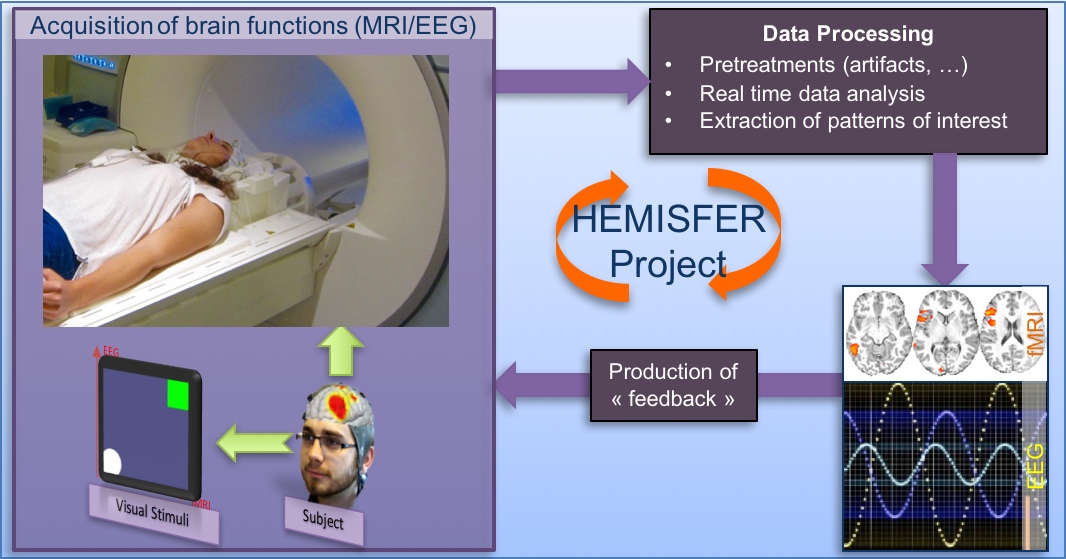
\includegraphics{IMG/Hemisfer_Principle.png}
        
        
        \subsubsection{France Life Imaging (FLI)}
        \begin{participants}    	
          \pers{Christian}{Barillot}, 	
          \pers{Olivier}{Commowick},
          \pers{Michael}{Kain},
          \pers{Florent}{Leray},
          \pers{Julien}{Louis},
          \pers{Aneta}{Morawin},
          \pers{Mathieu}{Simon},
          \pers{Yao}{Chi}
        \end{participants}  
        
        France Life Imaging (FLI) is a proposed large-scale research infrastructure
        project aimed at establishing a coordinated and harmonized network of
        biomedical imaging in France. This project was recently selected by the call
        ``Investissements d’Avenir - Infrastructure en Biologie et Santé''. One node of
        this project is the node Information Analysis and Management (IAM), a
        transversal node build by a consortium of teams that will contribute to the
        construction of a network for data storage and information processing. Instead
        of building yet other dedicated facilities, the IAM node will use already
        existing data storage and information processing facilities (LaTIM Brest;
        CREATIS Lyon; CIC-IT Nancy; VisAGeS U1228 Inria Rennes; CATI CEA Saclay;
        LSIIT/ICube Strasbourg) that will increase their capacities for the FLI
        infrastructure. Inter-connections and access to services will be achieved
        through a dedicated software platform that will be developed based on the
        expertise gained through successful existing developments.  The IAM node has
        several goals. It aims first at building a versatile facility for data
        management that will inter-connect the data production sites and data
        processing for which state-of-the-art solutions, hardware and software, will be
        available to infrastructure users. Modular solutions are preferred to
        accommodate the large variety of modalities acquisitions, scientific problems,
        data size, and adapted for future challenges. Second, it aims at offering the
        latest development that will be made available to image processing research
        teams.  The team VisAGeS fulfills multiple roles in this nation-wide project.
        Christian Barillot is the chair of the node IAM, Olivier Commowick is
        participating in the working group workflow and image processing and Michael
        Kain the technical manager. Apart from the team members, software solutions
        like MedInria and Shanoir will be part of the final software platform.
        
        
        %%% \subsection{Collaboration with the CEA (Commissariat à l'Energie Atomique):
        %%% Standardization of Arterial Spin Labeling acquisitions and imaging data quality
        %%% assessment in the context of dementia related studies}
        %%% \begin{participants}
        %%%   \pers{Élise}{Bannier}, 
        %%%   \pers{Christian}{Barillot}, 
        %%%   \pers{Isabelle}{Corouge},
        %%%   \pers{Jean-Christophe}{Ferré}, 
        %%%   \pers{Cédric}{Meurée}
        %%% \end{participants}
        %%% {\em duration: from August 2014 to December 2015}
        %%% 
        %%% Around 900,000 people are affected by various forms of dementia in France. As
        %%% an early and reliable diagnosis remains difficult to provide, neuroimaging is
        %%% crucial as a diagnosis assistance by analyzing structural and functional brain
        %%% abnormalities related to these diseases. The CATI (Centre pour l'Acquisition et
        %%% le Traitement des Images) is a multicenter neuroimaging network dedicated to
        %%% the management of dementia related imaging protocols. As VisAGeS and the
        %%% Neurinfo platform are recognized for their expertise in Arterial Spin Labeling
        %%% (ASL) acquisition and post-processing, a collaboration contract was signed
        %%% between Inria and CEA, the coordinator of the CATI initiative, in order to host
        %%% an engineer in the VisAGeS team for one year. The collaboration resulted in the
        %%% standardization of the ASL acquisition parameters of the CATI protocols, the
        %%% setup of these parameters on the scanneres participating in the CATI studies,
        %%% as well as the development and the integration of post-processing and quality
        %%% assessment tools into qualiCATI, the quality control software of the CATI.
        
        
        \subsubsection{OFSEP}
        \begin{participants}    	
          \pers{Élise}{Bannier},
          \pers{Christian}{Barillot}, 	
          \pers{Olivier}{Commowick},    	
          \pers{Gilles}{Edan},
          \pers{Jean-Christophe}{Ferré},
          \pers{Michael}{Kain},     
          \pers{Inès}{Fakhfakh}     
        \end{participants}
         
        The French Observatory of Multiple Sclerosis (OFSEP) is one of 10 projects
        selected in January 2011 in response to the call for proposal in the
        ``Investissements d’Avenir - Cohorts 2010'' program launched by the French
        Government. It allows support from the National Agency for Research (ANR) of
        approximately € 10 million for 10 years. It is coordinated by the Department of
        Neurology at the Neurological Hospital Pierre Wertheimer in Lyon (Professor
        Christian Confavreux), and it is supported by the EDMUS Foundation against
        multiple sclerosis, the University Claude Bernard Lyon 1 and the Hospices
        Civils de Lyon.  OFSEP is based on a network of neurologists and radiologists
        distributed throughout the French territory and linked to 61 centers. OFSEP
        national cohort includes more than 50,000 people with Multiple Sclerosis,
        approximately half of the patients residing in France. The generalization of
        longitudinal monitoring and systematic association of clinical data and
        neuroimaging data is one of the objectives of OFSEP in order to improve the
        quality, efficiency and safety of care and promote clinical, basic and
        translational research in MS.  For the concern of data management, the Shanoir
        platform of Inria has been retained to manage the imaging data of the National
        OFSEP cohort in multiple sclerosis.
        
        \end{module} 




%%%%%%%%%%%%%%%%%%%%%%%%%%%%%%%%%%%%%%%%%%%%%%%%%%%%%%%%%%%%%%%%%%%%%%
%%%
%%% Information sur les données importées : projets européens
%%%  
%%% Les données sur vos partenariats européens sont issus de la DPEI via l'entrepôt de données.  
%%% Les données affichées sont : Nom du projet, Type Defi, Instrument, Duration, Coordinator, Others partners.
%%%
%%% Complétez ce qui manque : résumé, Others partners (on attend des noms de pays), ...  
%%%
%%%Documentation intranet : https://intranet.inria.fr/Vie-scientifique/Information-edition-scientifiques/Comment-rediger-le-RAweb/Les-sections#eztoc27554_14
%%%
%%% En cas de problème : https://helpdesk.inria.fr/categories/181/submit
%%%
%%%%%%%%%%%%%%%%%%%%%%%%%%%%%%%%%%%%%%%%%%%%%%%%%%%%%%%%%%%%%%%%%%%%%%

\begin{module}{partenariat}{europe}{European Initiatives}

\subsection{FP7 \& H2020 Projects}
*TODO*


% %%%%%%%%%%%%%%%%%%%%%%%%%%%%%%%%%%%%%%%%%%%%%%%%%%%%%%%%%%%%%%%%%%%%%%%%%%%%%%
% % Donnees  construites d'après les informations de la base DPE pour 2018
% % Source : https://drone.inria.fr/
% % Date : jeudi 22 novembre 2018, 15:00:58 (UTC+0100)
% %




\subsection{Collaborations in European Programs, Except FP7 \& H2020}
% Eureka, COST...

% respecter le format  
%% \begin{itemize}
%% Gardez la ligne suivante :
%% \XMLaddatt*{type}{sanspuces}
%%         \item Program:
%%         \item Project acronym:
%%         \item Project title:
%%         \item Duration: mois ann\'ee d\'ebut - mois ann\'ee fin
%%         \item Coordinator:
%%         \item Other partners: organisme, labo (pays)
%%         \item Abstract:  
%% \end{itemize}

\begin{itemize}
\XMLaddatt*{type}{sanspuces}
        % \item Program:
        \item Project acronym: OpenAire-Connect
        \item Project title: OpenAire-Connect
        \item Duration: mois ann\'ee d\'ebut - mois ann\'ee fin
        \item Coordinator:
        \item Other partners: organisme, labo (pays)
        \item Abstract:  The OpenAire-Connect H2020 project will introduce and implement the concept of Open Science as a Service (OSaaS) on top of the existing OpenAIRE infrastructure, delivering out-of-the-box, on-demand deployable tools. OpenAIRE-Connect will adopt an end-user driven approach (via the involvement of 5 prominent research communities), and enrich the portfolio of OpenAIRE infrastructure production services with a Research Community Dashboard Service and a Catch-All Notification Broker Service. The first will offer publishing, interlinking, packaging functionalities to enable them to share and re-use their research artifacts (introducing methods, e.g., data,software, protocols). This effort, supported by the harvesting and mining “intelligence” of the OpenAIRE infrastructure, will provide communities with the content and tools they need to effectively evaluate and reproduce science. OpenAIRE-Connect will combine dissemination and training with OpenAIRE's powerful NOAD network engaging research communities and content providers in adopting such services. These combined actions will bring immediate and long-term benefits to scholarly communication stakeholders by affecting the way research results are disseminated, exchanged, evaluated, and re-used. In this project VisAGeS is acting, through CNRS, as the French coordinator to develop the link with the Neuroimaging research community. This will be performed in the context of the FLI-IAM national infrastructure.
\end{itemize}

OpenAire-Connect

The OpenAire-Connect H2020 project will introduce and implement the concept of Open Science as a Service (OSaaS) on top of the existing OpenAIRE infrastructure, delivering out-of-the-box, on-demand deployable tools. OpenAIRE-Connect will adopt an end-user driven approach (via the involvement of 5 prominent research communities), and enrich the portfolio of OpenAIRE infrastructure production services with a Research Community Dashboard Service and a Catch-All Notification Broker Service. The first will offer publishing, interlinking, packaging functionalities to enable them to share and re-use their research artifacts (introducing methods, e.g., data,software, protocols). This effort, supported by the harvesting and mining “intelligence” of the OpenAIRE infrastructure, will provide communities with the content and tools they need to effectively evaluate and reproduce science. OpenAIRE-Connect will combine dissemination and training with OpenAIRE's powerful NOAD network engaging research communities and content providers in adopting such services. These combined actions will bring immediate and long-term benefits to scholarly communication stakeholders by affecting the way research results are disseminated, exchanged, evaluated, and re-used. In this project VisAGeS is acting, through CNRS, as the French coordinator to develop the link with the Neuroimaging research community. This will be performed in the context of the FLI-IAM national infrastructure.

    Participants: Christian Barillot; Michael Kain; Camille Maumet

    Partners: PI: CNR, Italy; Athena Research And Innovation Center In Information Communication \& Knowledge Technologies, Greece; Uniwersytet Warszawski, Poland; JISC LBG, UK; Universitaet Bremen, Germany; Universidade Do Minho, Portugal; CNRS (Visages, Creatis), France; Universita Di Firenze, Italy; Institut De Recherche Pour Le Developpement (IRD), France; European Organization For Nuclear Research (CERN), Switzerland; International Center For Research On The Environment And The Economy, Greece

    Budget: 2M € (120k€ for CNRS)

Health

EIT Health aims to promote entrepreneurship and develop innovations in healthy living and active ageing, providing Europe with new opportunities and resources. EIT Health will enable citizens to lead healthier and more productive lives by delivering products, services and concepts that will improve quality of life and contribute to the sustainability of healthcare across Europe. EIT Health is a strong, diverse and balanced partnership of best-in-class organisations in education, research, technology, business creation and corporate and social innovation. EIT Health intends to foster cooperation and unlock Europe’s innovation and growth potential – developing and retaining the best talents, creating high-quality jobs and boosting the global competitiveness of European industry. VisAGeS is involved in this project through the Inserm and Inria institutions. Christian Barillot is representing Inria as one expert in the dedicated WG “Healthy Brain”. VisAGeS is also concerned by the WG “big data”.

    Participants: Christian Barillot, Michael Kain

    Partners: see https://www.eithealth.eu/partners



% organisation europeenne  
\subsection{Major European Organizations with which the Team have followed Collaborations}
*TODO*

\subsection{Collaborations with Major European Organizations}
*TODO*

% respecter le format
%%  \begin{itemize}
%%  \XMLaddatt*{type}{sanspuces}
%%         \item Partner 1: organisme 1, labo 1 (pays 1)
%%         \item Sujet 1 (max. 2 lignes)
%%  \end{itemize}
%%  \begin{itemize}
%%  \XMLaddatt*{type}{sanspuces}
%%        \item Partner 2: organisme 2, labo 2 (pays 2)
%%        \item Sujet 2 (max. 2 lignes)
%%  \end{itemize}


\end{module}


%%%%%%%%%%%%%%%%%%%%%%%%%%%%%%%%%%%%%%%%%%%%%%%%%%%%%%%%%%%%%%%%%%%%%%
%%%
%%% Information sur les données importées : équipes associées et autres actions internationales
%%%  
%%% La rubrique est partiellement pré-remplie avec les items suivants issus de la base de la DPEI.
%%% Les équipes associées engagées dans un IIL sont importées sous "Inria International Labs".
%%%  
%%% Vous devez compléter cette rubrique.
%%%  
%%% Inria International Labs  
%%% Associate Team not involved in an IIL
%%% Inria International Partners
%%%  A. Declared Inria International Partners
%%%  B. Informal International Partners
%%% Participation in other International Programs
%%% Pour vos collaborations internationales, précisez bien le nom anglais du pays en toutes lettres sauf pour les Etats-Unis (utilisez USA).
    
%%%Documentation intranet : https://intranet.inria.fr/Vie-scientifique/Information-edition-scientifiques/Comment-rediger-le-RAweb/Les-sections#eztoc27554_15
%%% Si vous voyez des erreurs, signalez-les via le  https://helpdesk.inria.fr/categories/181/submit
%%%%%%%%%%%%%%%%%%%%%%%%%%%%%%%%%%%%%%%%%%%%%%%%%%%%%%%%%%%%%%%%%%%%%%

\begin{module}{partenariat}{internationalInitiatives}{International Initiatives}

\subsection{Inria International Labs}
*TODO*

%%% Implication dans les activités des laboratoires conjoints à l'étranger  
%%% (Inria-Chile, JLESC, LIRIMA, LIAMA , Inria@SiliconValley, EPFL)
%%% Les équipes associées impliquées dans un IIL apparaissent ici :




%%% Ci-dessous, les projets rattachés à l'IIL hors les équipes associées
\subsubsection{Other IIL projects}
*TODO*




\subsection{Inria Associate Teams Not Involved in an Inria International Labs}
*TODO*


%%%%%%%%%%%%%%%%%%%%%%%%%%%%%%%%%%%%%%%%%%%%%%%%%%%%%%%%%%%%%%%%%%%%%%%%%%%%%%
% Donnees construites d'après les informations de la base DRI pour 2018
% Source : https://drone.inria.fr/
% Date : jeudi 22 novembre 2018, 15:00:58 (UTC+0100)
%






\subsection{Inria International Partners}
%%% indique un partenariat international important pour votre équipe,  
%%% hors Equipes Associées et hors participation aux programmes internationaux mentionnés ci-dessous

        \subsubsection{Declared Inria International Partners}
        *TODO*


%%%%%%%%%%%%%%%%%%%%%%%%%%%%%%%%%%%%%%%%%%%%%%%%%%%%%%%%%%%%%%%%%%%%%%%%%%%%%%
% Donnees construites d'après les informations de la base DRI pour 2018
% Source : https://drone.inria.fr/
% Date : jeudi 22 novembre 2018, 15:00:58 (UTC+0100)
%






        \subsubsection{Informal International Partners}
        
%%%        Vous pouvez écrire du texte

%%% Si les subsections précédentes sont vides utilisez plutôt le titre sans "Other" : Participation in International Programs
%%% au lieu de : Participation in Other International Programs
\begin{itemize}
    \item Collaboration with Neuropoly, Polytechnique Montreal: Haykel Snoussi visited the group of Julien Cohen-Adad and received an Inria-MITACS fellowship for a 3 months period (Nov. 2017-Jan. 2018). He worked on the processing of diffusion-weighted images of multiple sclerosis patients' spinal cord in the context of the EMISEP project.
\end{itemize}

\subsection{Participation in Other International Programs}
%%%   * Implication dans des activités avec des partenaires français :  JFLI ; IFCAM ; LICIA ; LIRIO ; ICeiRA
%%%   * Participation aux différents programmes soutenus par la DPEI et/ou des financeurs externes comme :
%%%   STIC AmSud, Math AmSud, STIC Asie, ECOS-Sud, IFCAM, autres...
*TODO*





\end{module}

\begin{module}{partenariat}{internationalVisitors}{International Research Visitors}
% Documentation intranet : https://intranet.inria.fr/Vie-scientifique/Information-edition-scientifiques/Comment-rediger-le-RAweb/Les-sections#eztoc27554_16

\subsection{Visits of International Scientists}
%chercheurs invités, profs invités (via université). Les internships sont à mettre dans la subsection suivante.

\begin{itemize}
    \item Alice Bates *TODO*
    \item Jean-Baptiste Poline *TODO*
\end{itemize}

   \subsubsection{Internships}
   *TODO*




\subsection{Visits to International Teams}
*TODO*
% Les explorateurs et sabbatiques provenant des bases de la DPEI sont importés dans votre trame.
% Vérifiez et complétez.
   \subsubsection{Sabbatical programme}
   *TODO*




   \subsubsection{Explorer programme}
   *TODO*




   \subsubsection{Research Stays Abroad}
   *TODO*
%% les séjours de chercheurs d'une durée supérieure à un mois, dans une université ou un laboratoire étranger




%XFYZ_IN_IN

%% ICI Vous pouvez ecrire du texte

\end{module}


%%%%%%%%%%%%%%%%%%%%%%%%%%%%%%%%%%%%%%%%%%%%%%%%%%%%%%%%%%%%%%%%%%
%%%
%%% Section diffusion des resultats (Dissemination)
%%% Il y a des modules ici
%%%
%%%%%%%%%%%%%%%%%%%%%%%%%%%%%%%%%%%%%%%%%%%%%%%%%%%%%%%%%%%%%%%%%%


\begin{module}{diffusion}{animation}{Promoting Scientific Activities}

%%% Le module "Promoting Scientific Activities" comprend les activités éditoriales,
%%% notamment de reviewing, d'organisation de conférences, de participation à des programmes de conférences.  
%%% Documentation intranet : https://intranet.inria.fr/Vie-scientifique/Information-edition-scientifiques/Comment-rediger-le-RAweb/Les-sections#eztoc27554_17

%%  respecter le format :  

\subsection{Scientific Events Organisation}
    \subsubsection{General Chair, Scientific Chair}
    \begin{itemize}
        \item MS workshop: \url{https://project.inria.fr/msworkshop2018/}, Jan 30-31, London, UK (Claire Cury).
        \item Brainhack Global Rennes 2018: \url{https://brainhack.irisa.fr}, May 25-26, Rennes, France (Camille Maumet).
    \end{itemize}    
    
%%%   si liste, alors merci d'utiliser :
%%%  \begin{itemize}
%%%     \item  
%%%     \end{itemize}    

    \subsubsection{Member of the Organizing Committees}
    \begin{itemize}
        \item Brainhack Global Rennes 2018: \url{https://brainhack.irisa.fr}, May 25-26, Rennes, France (Julie Coloigner, Olivier Commowick, Claire Cury, Mathis Fleury).
	\item MS workshop: \url{https://project.inria.fr/msworkshop2018/}, Jan 30-31, London, UK (Christian Barillot).
    \end{itemize}    
    \subsubsection{Program Participant}
    \begin{itemize}
        \item Organizer of the project 'A deep learning playground', Brainhack Global Rennes 2018: \url{https://brainhack.irisa.fr}, May 25-26, Rennes, France (Francesca Galassi).
    \end{itemize}  
\subsection {Scientific Events Selection}
    \subsubsection{Chair of Conference Program Committees}
    *TODO*
    \subsubsection{Member of the Conference Program Committees}
    \begin{itemize}
        \item Scientific commitee of SFRMBM 2019, bi-annual congress that will be help in Strasbourg in March 2019 \url{https://sfrmbm2019.sciencesconf.org/} (Elise Bannier).
        \item Neuroinformatics 2019: \url{neuroinformatics2019.org/}, Sept. 1-2, Warsaw, Poland (Camille Maumet).
    \end{itemize}
    \subsubsection{Reviewer}
    \begin{itemize}
        \item International Symposium on Medical Information Processing and Analysis: ISBI (Julie Coloigner, Olivier Commowick, Pierre Maurel)
        \item MICCAI (Olivier Commowick, Francesca Galassi)
        \item IPMI (Olivier Commowick)
        \item African Conference on Research in Computer Science and Applied Mathematics (CARI) (Pierre Maurel)
    \end{itemize}   
\subsection{Journal}
    \subsubsection{Member of the Editorial Boards}
    \begin{itemize}
        \item Neuroinformatics (Camille Maumet)
    \end{itemize}   
    \subsubsection{Reviewer - Reviewing Activities}
    \begin{itemize}
        \item Journal of Alzheimer's disease (Claire Cury)
        \item NeuroImage (Olivier Commowick, Pierre Maurel, Camille Maumet)
        \item NeuroImage: Clinical (Julie Coloigner)
        \item IEEE TMI (Olivier Commowick)
        \item Med Image Anal (Olivier Commowick)
    \end{itemize}    
\subsection{Invited Talks}
\begin{itemize}
    \item C. Barillot, O.Commowick. ``Objective Evaluation of Multiple Sclerosis Lesion Segmentation using a Data Management and Processing Infrastructure'' - Journées françaises de radiologie - Paris (Oct 2018)~\cite{commowick:inserm-01895603}
    \item O.Commowick. ``Objective Evaluation of Multiple Sclerosis Lesion Segmentation using a Data Management and Processing Infrastructure''. France Life Imaging workshop - Orsay (March 2018)
    \item O. Commowick ``Towards Multiple Sclerosis Lesions Segmentation Transfer to the Clinics: Methods and Evaluation''. Gdr ISIS - Paris (March 2018)
    \item In the context of the EMISEP project on MS and spinal cord imaging and in order to discuss further collaboration, Anne Kerbrat, Benoit Combès and Elise Bannier visited the CEMEREM in Marseille on Monday and gave a talk `` Characterisation of spinal cord involvement in early RRMS patients using MRI'' (October 22st)
    \item C. Maumet ``Tools and standards to make neuroimaging derived data reusable'', Keynote at Neuroinformatics 2018, Montreal, Canada, August 2018~\cite{maumet:inserm-01886089}.
\end{itemize}


\subsection{Leadership within the Scientific Community}
\begin{itemize}
    \item Chair-elect of the international OHBM Open Science Special Interest Group (Camille Maumet)
    \item Member of the international working group on data sharing in neuroimging of the International Neuroinformatics Coordinating Facility (Camille Maumet)
    \item Member (by invitation) of Aperture, an international new online publishing plateform for the OHBM community, in the ``workflow working group'' led by Peter Bandettini  (Camille Maumet).
    \item Member (by selection) of the ``comité de la science ouverte'', a national initiative to foster open science in France, in the ``open and free software working group'' led by Roberto Di Cosmo  (Camille Maumet).
    \item Mentor (by selection) of the international training ``Mozilla Open leaders'' led by Abigail Cabunoc Mayes (Camille Maumet).
\end{itemize}    
\subsection{Scientific Expertise}
*TODO*
\subsection{Research Administration}
*TODO*
  
\end{module}


\begin{module}{diffusion}{enseignement}{Teaching - Supervision - Juries}

\subsection {Teaching}

\begin{itemize}
\XMLaddatt*{type}{sanspuces}
     \item Cédric Meurée, Algorithms and Complexity, 28h, M1, ESIR, France
     \item Corentin Vallée, Machine Learning, 64h, M1, Univ. Rennes, France
     \item Raphaël Truffet, Génie Logiciel, 24h, L2, ISTIC, France
     \item École Supérieure d’Ingénieur de Rennes (ESIR): Pierre Maurel, General image processing (60h), Algorithmics and complexity (60h), Medical imaging (60h)
    \item ENS Rennes: Pierre Maurel, Introduction to image processing (24h)
    \item Pierre-Yves Jonin, Introduction aux méthodes de neuroimagerie pour la recherche en neuropsychologie (3h) Master 2. Université de Poitiers, France.
    \item Pierre-Yves Jonin,Evaluation neuropsychologique à visée diagnostique. Le cas des syndromes démentiels. Master 2 (2 x 6h) Université de Poitiers, France.
    \item Pierre-Yves Jonin,L'exploration neuropsychologique des maladies neurologiques et psychiatriques. 4\`eme \& 5\`ame année de m\'edecine (4h), Universit\'a de Brest, France.
    \item Pierre-Yves Jonin, Neurosciences cognitives de la mémoire humaine. Master 2. 3 heures. Université de Rennes 1, France.
    \item Pierre-Yves Jonin, Les syndromes neuropsychologiques. Licence 3, (16h) Université de Rennes 2, France
    \item Pierre-Yves Jonin, L'approche neuropsychologique du handicap chez les patients cérébro-lésés. Licence 3. Université de Rennes 2.
    \item Pierre-Yves Jonin, Evaluation neuropsychologique à visée diagnostique. Le cas des syndromes démentiels. Master 2. 2 x 6 heures. Université de Rennes 2.
    \item Pierre-Yves Jonin, Méthodologie de la recherche clinique. Master 2. 3 heures. Université de Rennes 2.
    \item Pierre-Yves Jonin, Méthodologie clinique et principes de l’évaluation neuropsychologique à visée diagnostique. Master 2. 3h30. Université de Savoie.
    \item Antoine Legouhy, Bio-statistques 34h, L2 biologie, Univ. Rennes 1, France.
    \item Antoine Legouhy, Optimisation 12h, M1 mathématiques, Univ. Rennes 1, France.
    \item Mathis Fleury, Mathématiques; 64h (3 months); Licence; IUT saint-Malo, France.
    \item Francesca Galassi, L1 INF1 : Programming in Java (TD : 20h, TP : 20h), ISTIC University of Rennes 1, France.
    \item Francesca Galassi, L2 PO : Object Oriented Programming in Java (TP : 20h), ISTIC University of Rennes 1.
    \item Master SIBM: Olivier Commowick, M2, University of Angers-Brest-Rennes (Plenary: 6h), France.
    \item Master SIBM: Quentin Duché, ``Traitements des données d'IRM fonctionnelle'', M2, University of Angers-Brest-Rennes (Plenary: 1h), France.
    \item Master SIBM: Isabelle Corouge, ``Bio marqueurs d’imagerie et IRM metabolique et fonctionnelle'', M2, University of Angers-Brest-Rennes (Plenary: 3h), France.
    \item Master SIBM: Camille Maumet, M2, University of Angers-Brest-Rennes (Plenary: 3h), France.
    \item Master SIBM: Élise Bannier, ``IRM fonctionnelle BOLD'' M2, University of Angers-Brest-Rennes (Plenary: 3h), France.
 \end{itemize}

%% Ce modulef présente vos activités d'enseignement et d'encadrement à présenter comme suit :

% respecter le format :  
 %%\begin{itemize}
  %%\XMLaddatt*{type}{sanspuces}
         %%\item Licence : Enseignant, titre du cours, nombre d'heures en équivalent TD, niveau (L1, L2, L3), université, pays  
         %%\item Master : Enseignant, titre du cours, nombre d'heures en équivalent TD, niveau (M1, M2), université, pays  
         %%\item Doctorat : Enseignant, titre du cours, nombre d'heures en équivalent TD, université, pays
         %%\end{itemize}

%%%
%%% Exemple de section E-learning à décommenter si besoin
%%%  
%       \begin{itemize}
%         \XMLaddatt*{type}{sanspuces}
%         \item \textbf{E-learning}  
%         \begin{itemize}
%         \XMLaddatt*{type}{sanspuces}
%                \item Mooc, SPOC, etc. : Enseignant ou auteur, titre du cours, durée en nombre de semaine, plate-forme, établissement porteur du cours, public ciblé, formation initiale ou continue, nombre d'inscrits
%                \item Pedagogical resources : enseignant, titre, type (video, pdf, exercice, ou autre), niveau, url
%         \end{itemize}    
% \end{itemize}
%

%%% Détaillez les activités d'enseignement au moins pour les chercheurs Inria permanents et les enseignants-chercheurs permanents.

\subsection {Supervision}
%% PhD \& HdR : Les thèses soutenues doivent figurer dans la bibliographie

 %%\begin{itemize}
  %%\XMLaddatt*{type}{sanspuces}
           %%\item HdR : nom du chercheur, titre du mémoire, nom de l'Université, date de soutenance
           %%\item PhD : nom du doctorant, titre du mémoire, nom de l'Université, date de soutenance, encadrant(s)
           %%\item PhD in progress : Nom du doctorant, titre (provisoire) du mémoire, date du début de la thèse, encadrant(s)
  %%\end{itemize}
 \subsubsection{PhD \& HdR}
 \begin{itemize}
  \XMLaddatt*{type}{sanspuces}
           \item PhD in progress: Cédric Meurée, ``''Quantitative Analysis Of Arterial Spin Labeling MRI For Robust Parametric Information Of Perfusion Maps'', Inria / Siemens, from Mar 2014, Christian Barillot, Pierre Maurel.
           \item PhD in progress : Corentin Vallée, "Joint estimation of neuronal activation, resting-state and basal metabolism from Arterial Spin Labeling", Univ. Rennes, from Nov 2016, Christian Barillot, Isabelle Corouge, Pierre Maurel.
           \item PhD in progress : Anne-Claire Binter, "Etude des effets possibles des expositions prénatales à des neurotoxiques (solvants organiques et insecticides organophosphorés) sur le fonctionnement du cerveau de l’enfant évalués par imagerie cérébrale (Cohorte Pélagie)", Univ. Rennes, from Janv 2017, Fabienne Pelé, Cécile Chevrier, Elise Bannier.
  \end{itemize}

  \subsubsection{Other supervisions}
  \begin{itemize}
  \XMLaddatt*{type}{sanspuces}
           \item Master student: Solene Tarride, ``''Deep learning for segmentation of MS lesions from multimodal MRI'', Apr-Oct 2018, Francesca Galassi.
  \end{itemize}

\subsection {Juries}
\begin{itemize}
    \item Isabelle Corouge, PhD mid-term committee (CSI) : Cédric Meurée, Rennes; May 2018.
    \item Élise Bannier, PhD mid-term committee (CSI) : Haykel Snoussi, Rennes; May 2018.
    \item Élise Bannier, PhD mid-term committee (CSI) : Louis Marage, Rennes; July 2018.
\end{itemize}

%% ICI Vous pouvez ecrire du texte dans le module

\end{module}

\begin{module}{diffusion}{popularization}{Popularization}

%%% Le module "Popularization"
%%% La médiation scientifique concerne toutes les actions à destination de publics sortant du cercle professionnel habituel des scientifiques :
%%% enfants et jeunes, curieux de la science, grand public, décideurs politiques et partenaires socio-économiques.
%%% La médiation fait intervenir le chercheur, auteur du contenu scientifique.

%% Organisez vos informations selon les catégories suivantes :

\subsection{Internal or external Inria responsibilities}
%%% Il s'agit de responsabilités collectives : chargé.e de mission, de médiation, membre de commissions (locales/nationales),  
%%% de comité éditorial de revues (interstices, images de maths, etc.), de comité scientifique de fondations,
%%% d'édition d'ouvrages de vulgarisation collectifs, ...
*TODO*

\subsection{Articles and contents}
 %%\begin{itemize}
       %%\item In books/journals for the general public
       %%\item For online publications (Interstices*, Images des Maths, Binaire, Wikipedia), and more widely blog articles
       %%\item Interviews in order to popularize
       %%\item White Papers - white Papers for Popularization
  %%\end{itemize}
%%% *Interstices articles are automatically entered into Hal
\begin{itemize}
   \item Camille Maumet: Blog post ``Open science working group on scientific sofware'' \url{http://blog.camillemaumet.com/posts/12}, November, personal website. 
   \item Elise Bannier: Blog post ``Village des sciences 2018'' \url{https://team.inria.fr/visages/village-des-sciences-2018/}, October, VisAGeS blog.  
   \item Camille Maumet: Blog post ``Extending BIDS to fMRI analyses'' \url{http://blog.camillemaumet.com/posts/posts/11}, October, personal website. 
   \item Olivier Commowick: Blog post: ``Anima scripts release'' \url{https://team.inria.fr/visages/anima-scripts-release/}, September, VisAGeS blog.
   \item Camille Maumet: Blog post ``Collaborative AFNI projects at DC code convergence'' \url{http://blog.camillemaumet.com/posts/10}, September, personal website. 
   \item Camille Maumet: Blog post ``Meeting Montreal neuroinformatics community at the INCF congress and hackathon'' \url{http://blog.camillemaumet.com/posts/9}, August, personal website. 
   \item Camille Maumet: Blog post ``Mentoring for Mozilla Open Leaders'' \url{http://blog.camillemaumet.com/posts/8}, August, personal website. 
   \item Camille Maumet with Claire Cury: Blog post ``Interview: Let’s organise a Brainhack!'' \url{https://team.inria.fr/visages/interview-lets-organise-a-brainhack/}, July, VisAGeS blog.
   \item Camille Maumet with Elise Bannier: Blog post ``Interview: Participating in my first hackathon at Brainhack Rennes 2018'' \url{https://team.inria.fr/visages/participating-in-my-first-hackathon-at-brainhack-rennes-2018/}, July, VisAGeS blog.
   \item Camille Maumet: Blog post ``OHBM 2018: first remotely-attended conference'' \url{http://blog.camillemaumet.com/posts/7}, June, personal website.
   \item Camille Maumet: Blog post ``Sprinting with bio-imagers and how I learnt about NEUBIAS, EuBI, Elixir and tried out myBinder!'' \url{http://blog.camillemaumet.com/posts/6}, May, personal website. 
   \item Olivier Commowick: Blog post ``Anima v3.0 release'' \url{https://team.inria.fr/visages/anima-v3-0-release/}, March, VisAGeS blog.
   \item Claire Cury: Blog post ``Workshop Multiple Sclerosis 2018 (UCL, Inria)'' \url{https://team.inria.fr/visages/workshop-multiple-sclerosis-2018-ucl-inria/}, April, VisAGeS blog.
   \item Olivier Commowick: Blog post ``Brainhack Rennes 2018 (April 25-26)'' \url{https://team.inria.fr/visages/brainhack-rennes-2018-april-25-26/}, March, VisAGeS blog.
   \item Olivier Commowick: Blog post ``medInria 3.0 available'' \url{https://team.inria.fr/visages/medinria-3-0-available/}, March, VisAGeS blog.
 \end{itemize}

\subsection{Education}
%%% *Interactions avec l'Education Nationale ou les structures d'éducation populaire
%%% (exemple : contribuer à former des formateurs,  participer à la transmission d'outils pédagogiques sur la pensée informatique,
%%% de personnels de l'Education Nationale ou de structures d'éducation populaire, par exemple en temps présentiel de Class'Code,
%%% ou encore des actions pour l'enseignement comme la participation à l'élaboration des programmes scolaires, interactions avec le CNNum, etc.)
%%% *Mise en place de modules doctoraux sur la médiation
%%% *Participations à/créations de Moocs dont on indiquera ici les enjeux de médiation (en complément de la section e-learning dans laquelle ce même Mooc devrait apparaître aussi)
%%% *Créations de cours (par exemple ISN)
%%% *Organisation de/participation à des salons à destination des professionnels de l'éducation (ORME, educatec-educatice....)
\begin{itemize}
    \item L codent L créent - An outreach program to send PhD students to teach Python to middle school students in 8 sessions of 45 minutes. Tassadit Bouadi (Univ. Rennes 1), Camille Maumet (VisAGeS) and Anne-Cecile Orgerie (Myriads) are coordinating the local version of this program, initiated in Lille. The first session in Rennes is planned for April 2019. The program is currently supported by: Fondation Blaise Pascal, ED MathSTIC, Inria and Fondation Rennes 1.
\end{itemize}

\subsection{Interventions}
 %%\begin{itemize}
    %%\item National events: Fête de la Science, Codeweek, Semaine des maths, one-off events such as Pint of Science
    %%\item Public exhibitions (Futurs en Seine,...)
    %%\item In educational institutions
    %%\item Welcoming of schoolchildren or the general public in an Inria center: MathC2+ internship, open days,...
  %%\end{itemize}


\subsubsection{National brain week: ``Semaine du Cerveau''}
\begin{itemize}
    \item Giulia Lioi: Talk ``Lire dans son cerveau grâce au neurofeedback EEG, c’est mieux bouger'', March 14, Warpzone, Rennes, France. 
    \item Mathis Fleury: Bar en (neuro) sciences; May 14-16; Presentation of the Neurofeedback and demonstration of a EEG based Neurofeedback with a motor imagery paradigm. 
\end{itemize}

\subsubsection{National science week: ``Village des sciences''}
Visages took part in the Village des Sciences 2018, opening the Neurinfo plateform to 45 middle school students (Oct 5) and 120 visitors from the general public (Oct 6-7), Oct 5-7, Rennes, France. \url{https://www.univ-rennes1.fr/evenements/20072018/village-des-sciences-2018-visites-guidees-de-laboratoires-pour-les-scolaires}, \url{https://team.inria.fr/visages/members-area/projects/village-des-science-2018/}. The event was coordinated by Julien Le Bonheur from the University of Rennes, and Elise Bannier coordinated the contribution of Neurinfo/Visages. We covered 4 themes: 
\begin{itemize}
        \item Giulia Lioi, Mathis Fleury, Simon Butet, Pauline Rolland: Neurofeedback EEG
        \item Pierre Maurel, Charlélie Erhart, Antoine Legouhy, Corentin Vallée, Francesca Galassi, Julie Coloigner: Image processing with MedInria
        \item Isabelle Corouge, Catherine Guillemot, Emmanuel Caruyer, Elise Bannier, Benjamin Parat: Brain and MRI
        \item Quentin Duché, Florian Chapelain, Virginie Dardier: Functional MRI
\end{itemize}

\subsubsection{Other interventions}
\begin{itemize}
    \item Pierre-Yves Jonin: Series of 6 talks on neuropsychology, Universités du Temps Libre de Bretagne, Jan-Dec, Rennes, France. 
    \item Pierre-Yves Jonin: Talk ``La mémoire humaine, comment la conserver, quand s’inquiéter'', Bien Vieillir en Ille-et-Vilaine, June, Rennes, France. 
    \item Mathis Fleury: Talk ``Qu'est ce qu'un doctorant ?''Journée des métiers IUT rennes - , Nov 16, IUT Rennes, France.
    \item Camille Maumet: Talk to middle school students  (around 100) ``La neuroinformatique'', PRNB, April, Rennes, France.
    \item Olivier Commowick: Presentation of research done in VisAGeS on medical image processing and of the MedInria software, Journée LOGIN, Nov 27, Grenoble, France. 
\end{itemize}

    
\subsection{Internal action}
*TODO* --> nothing?
 %%\begin{itemize}
     %%\item Internal meetings such as Café des sciences
     %%\item Training of colleagues on new contents or media (activités débranchées, Poppy Ergo, TensorFlow,...)
     %%\item Training follow-up (Media Training, new media such as Poppy ergo, with SIF, etc.)
     %%\item Science outreach towards services (DPEI, STIP...)
  %%\end{itemize}

\subsection{Creation of media or tools for science outreach}
%%% Nouveaux supports pour comprendre les fondamentaux des sciences du numérique ou
%%% pour expliquer des résultats de recherche des plus ancrés aux plus récents :
%%% vidéos, slides, création de jeu (qui explique un sujet, par exemple : Model checking), fiches autonomes d'activités, …
\begin{itemize}
    \item Launching of a Twitter account for the VisAGeS team (Camille Maumet) and setup on the VisAGeS website (Olivier Commowick)~\url{http://twitter.com/inria_visages}. Tweets by lab members (Quentin Duché, Christian Barillot)
    \item Development of the VisAGeS blog and writing of blog posts (Camille Maumet, Olivier Commowick, Claire Cury, Elise Bannier).
\end{itemize}


\end{module}


%%%%%%%%%%%%%%%%%%%%%%%%%%%%%%%%%%%%%%%%%%%%%%%%%%%%%%%%%%%%%%%%%%%%
%%%
%%% Section bibliographie
%%%
%%% Il y a trois fichiers de bibliographie
%%%
%%% - visages_refer2018.bib est inclus dans sa totalité mais en commentaire, sélectionnez les 10
%%%   références majeures du projet en les décommentant (Remplacer AROBAS par @). Pour les citer : \refercite
%%%
%%% - visages2018.bib les publis de l'année 2018 issues de Hal, citées par \cite
%%%
%%% - visages_foot2018.bib contient les citations utilisées en note  de bas de page, citées par \footcite  
%%%
%%% Vérifier si les noms des auteurs sont corrects  
%%%
%%%
%%%%%%%%%%%%%%%%%%%%%%%%%%%%%%%%%%%%%%%%%%%%%%%%%%%%%%%%%%%%%%%%%%%%%%

%%%%%%%%%%%%%%%%%%%%%%%%%%%%%%%%%%%%%%%%%%%%%%%%%%%%%%%%%%%%%%%%%%%%%%
%%%
%%% Information sur les données exportées : biblio
%%%  
%%% Seules les publications présentes dans Hal seront prises en compte dans le RA 2018 comme publications de l'année.
%%% Lors de la compilation sur iRabot le fichier visages2018.bib sera automatiquement récupéré à partir de Hal.  
%%% Le fichier visages2018.bib ne doit pas être édité.
%%%
%%% Vous devez donc déposer dans Hal https://hal.inria.fr/ vos publications manquantes.  
%%% Attention, pour  cause de validation, il peut y avoir un délai de 24h avant la mise en ligne et l'intégration à la trame.  
%%% Les thèses soutenues doivent figurer dans la biblio et donc être sur Hal.
%%%
%%% Consulter la bibliographie de l'année : https://irabot.inria.fr/itramera?&format=bib&epi=visages&annee=2018
%%%
%%%Rappel : les Best papers cités en section Highlights sont affichés dans la biblio sur fond de couleur avec la mention "Best paper".
%%%Citez les publications récompensées sous la forme : \bestcite{xxxx}, \bestcite{yyyy}.

%%% Les publications de référence et celles en notes de bas de pages sont issues de votre RAweb 2017
%%% Url de consulation du RAweb 2017 : http://raweb.inria.fr/rapportsactivite/RA2017/index.html
%%%
%%% Depuis le 25/09/2018, vous pouvez déposer du code source dans HAL et ainsi contribuer au patrimoine logiciel constitué par Software Heritage.
%%% La notice logiciel de Hal est affichée en catégorie misc.

%%% Vérifiez et signalez erreurs et problèmes  via le  https://helpdesk.inria.fr/categories/181/submit
%%%
%%%%%%%%%%%%%%%%%%%%%%%%%%%%%%%%%%%%%%%%%%%%%%%%%%%%%%%%%%%%%%%%%%%%%%

%%% Attention, il n'y a pas de \nocite{*} implicite.  
%%% Une commande \nocite{*} a été ajoutée.
%%% Vous pouvez utiliser des \nocite{xx}.
%   \nocite{TFE98}
%   \nocite{AGATHISC}
%   \nocite{FD98}
%   \nocite{x,y,z}  

%%% Une commande \omitcite a été créée pour permettre d'exclure certaines références de publication Hal de la biblio du RA.
%%% Syntaxe : un omitcite par ligne
%%%    \omitcite{bret:hal-00000}
%%%    \omitcite{bret:hal-00000}
%%%    \nocite{*}

\nocite{*}
\loadbiblio

%%%%% fin du document
\end{document}


%% VISAGES
%% Date : jeudi 22 novembre 2018, 15:00:58 (UTC+0100)
%% Source rapport latex VISAGES : http://ralyx.inria.fr/Raweb/visages/uid0.html
%% Source donnees bastri SR0103YR : https://bastri.inria.fr/Bastri/structureinria/siid/SR0103YR/look
%% Source donnees bil VISAGES : https://bil.inria.fr/
